\documentclass[12pt,upcase]{umlthesis}
\usepackage{lipsum}
\usepackage{natbib}
\usepackage{graphicx}
\usepackage{float}
\usepackage{hyperref}
\usepackage{amsmath}
\usepackage{amssymb}
\usepackage{booktabs}

\def\code#1{\texttt{#1}}
% use fancyhdr, to enable page style stuff (below)
\usepackage{fancyhdr}
\setlength{\headheight}{15.2pt}
\renewcommand{\headrulewidth}{0pt}

\pagestyle{plain}

\begin{document}
\title{Two-Fluid Collisional Magnetohydrodynamic Modeling}
\author{Qusai Al Shidi}
\prevdegrees{B.S., University of Toledo (2008)}
\department{Department of Physics and Applied Physics}
\degree{Doctor of Philosophy}
\degreemonth{May}
\degreeyear{2019}
\thesisdate{May 1, 2019}
\supervisor{Ofer Cohen}{Assistant Professor}
\maketitle

%%%%%%%%%%%%%%%%%%%%%%%%%%%%%%%%%%%%%%%%
\begin{abstract}
	Since the discovery of space plasmas, the space science community have been deriving fluid models of plasmas to best suit their scenarios. The simplest case is the ideal magnetohydrodynamic (MHD) model which assumes a collisionless perfectly-conducting plasma. Multi-fluid collisional MHD gives each fluid its own set of MHD equations while using collisions to set frictional and resistive terms between them. An important case of this nature is the solar chromosphere. The high density and relatively cold plasma ensures collision times are shorter than magnetic time scales. Multi-fluid collisional MHD has many cases from the Earth's ionosphere to stellar atmosphere and having a good grasp of the physics is important in studying these plasmas.
\end{abstract}
%%%%%%%%%%%%%%%%%%%%%%%%%%%%%%%%%%%%%%%%
\chapter*{Acknowledgements}
To my partner Alexis Ploss, who believed in me without judgment or apprehension. To my family, that supported me beyond the ocean. To my dog Ada Lovelace, that provided emotional support through the hardships.


%%%%%%%%%%%%%%%%%%%%%%%%%%%%%%%%%%%%%%%%
\tableofcontents
\listoffigures
\listoftables

\chapter{Introduction}

The word `plasma' was first used by \citet{Langmuir1928} to describe oscillations in a gaseous electron medium~\citep{Tonks1967}. It is a state of matter that is can be described as an ionized gas. It is the most common form of baryonic matter in the universe. We default to plasma descriptions of the medium between stars and planets. The sun is, for example, made mostly of ionized hot plasma. It is made of plasma and shoots out supersonic plasma called the solar wind. This plasma does not entirely contact the Earth due to shielding resulting from the Earth's magnetic field. Due to plasma's ionization, it has a tendency to travel on magnetic field lines. This does not mean the Earth is completely shielded from the solar wind. Many space weather events are due to solar plasma's effect on the Earth and its magnetic field. The sun is a very active star that has spontaneous flares, coronal mass ejections (CME) and active regions. Thus spontaneous storms occur on Earth and our understanding of the sun and space plasmas is essential to protect ourself against storms.

In this dissertation, an attempt will be made to show the benefits and utility of multi-fluid magnetohydrodynamic (MHD) models. We will show that the solar chromosphere is a good case for this. The implementation will also be studied with careful use of good, modern computer science practices.

\section{The Sun}

\begin{figure}[h!]\label{fig:sunstructure}
	\centering
	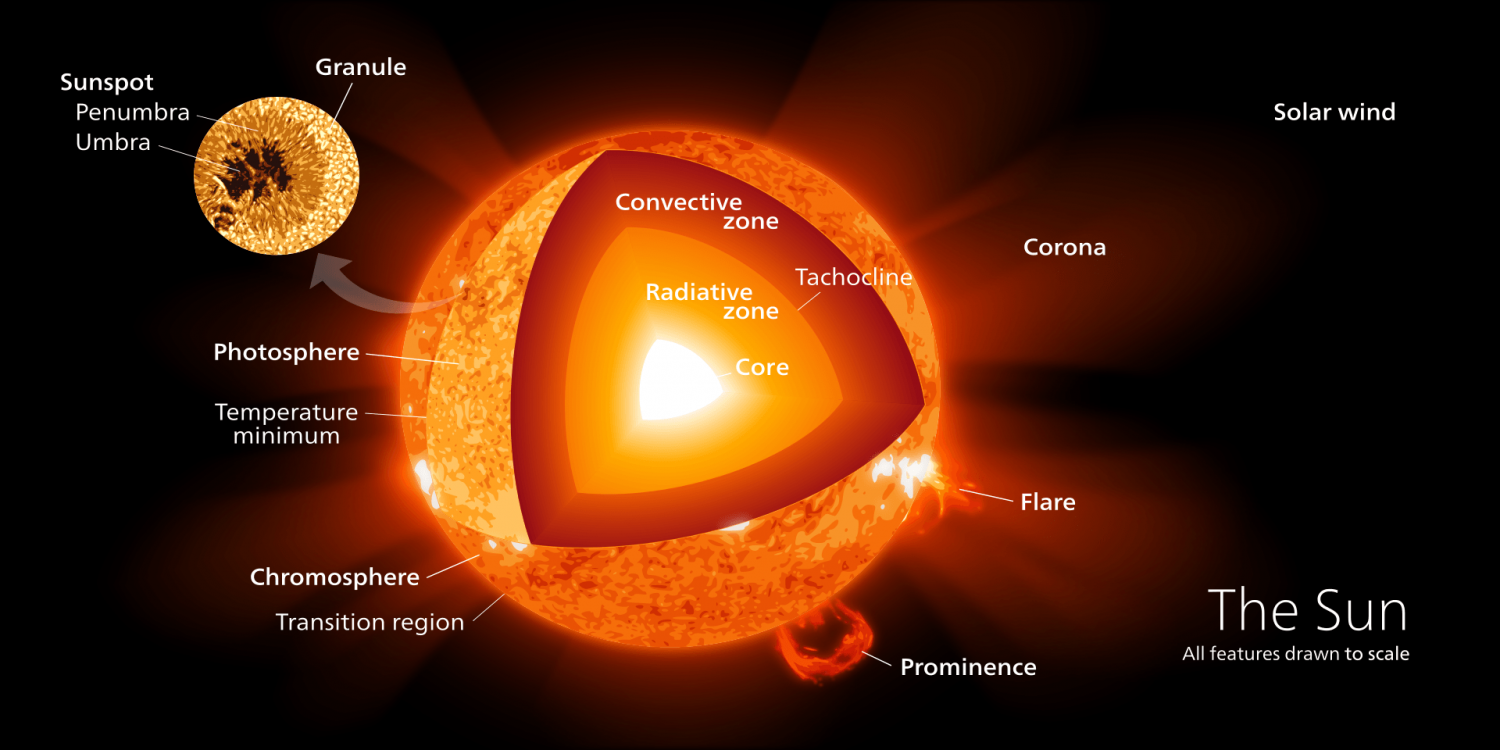
\includegraphics[width=1.0\linewidth]{images/sunstructure.png}
	\caption{A more complicated view of the sun's structure and layers. [{Image from \url{https://phys.org/news/2015-12-sun-energy.html}}]} % chktex 8
\end{figure}

Whenever I say `the sun' I do not mean any star---I mean \textit{our} star. The sun is a 4.6 billion year old yellow dwarf. It generates a lot of the energy we use for life on Earth. It creates this energy through nuclear fusion in its core, turning hydrogen into helium. The sun is mostly hydrogen with a small amount of helium and even smaller amounts of metal ions which require tremendous energy to fuse. The sun has six regions (from innermost to outermost): the core, the radiative zone, the convection zone, the photosphere, the chromosphere and the corona. The core is where the fusion happens. Here is where hydrogen is made into helium and other metals. The radiative zone and convection zone is where the energy travels radially upwards to wards the surface, the photosphere. The photosphere is the surface of the Sun. Here photons are trapped but the ones that do escape mimic black-body radiation (not perfectly). It is optically thick and is the white light we see when looking at the Sun. Above the photosphere is the atmospheric layer, the chromosphere, which I will go in much detail about in this dissertation. Above that, is the corona which is what gives the sun its tendrils and the hair we give our cartoon drawings of the sun.

\subsection{The Chromosphere}

The chromosphere is the interface between the surface, the photosphere, and the outer atmosphere, the corona. The plasma in it is partially ionized which means it consists of two kinds of plasma: ionized (charged) plasma, and neutral (uncharged) plasma. This means the charged plasma is affected by Lorentz forces while the uncharged plasma is not. This is a result of the temperature of the chromosphere and the composition of the plasma convected in the convection zone. The plasma has a high temperature in Earth standards but to the sun it is relatively cold. The temperature of the corona, which keep in mind is the outermost layer, is in the million of degrees in Kelvin. While most of the chromosphere and the photosphere is 5000K-6500K. This discrepancy in the temperature of the lower layers to the higher layers is called the coronal heating problem. The coronal heating problem is an outstanding problem in physics which makes understanding the chromosphere of special importance. Why is the corona hotter than the chromosphere?

\begin{figure}[ht!]\label{fig:chromoprofile}
	\centering
	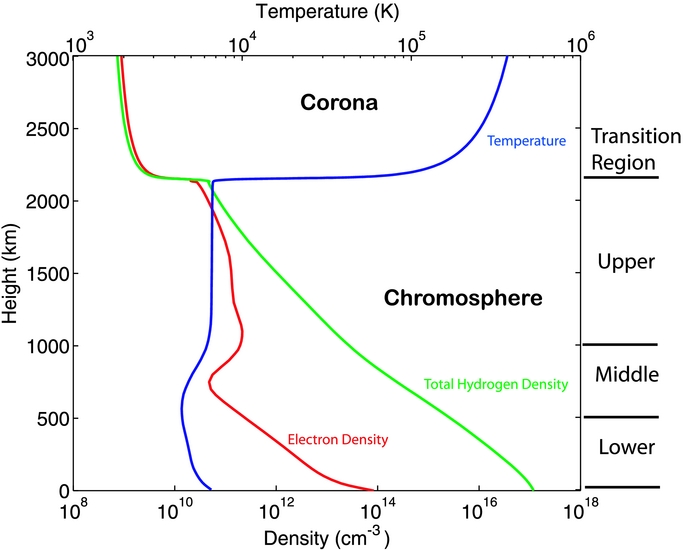
\includegraphics[width=0.75\linewidth]{images/chromoprofile.jpg}
	\caption{A view of the upper, middle and lower chromosphere. The chromosphere is partially ionized and is much colder than the corona (above the transition region).~\citep{Song2014,Avrett2008}}
\end{figure}


\section{Space Weather}

The term space weather refers to weather effects found above our immediate atmosphere which is conversely named terrestrial weather. It focuses on the conditions and changes found between the Sun, the Earth and even behind the Earth along its night time. The Earth's surface magnetic field strength is in the 0.5G range~\citep{Finlay2010} and that is strong enough to shield most of the solar wind headed our direction. However, magnetic reconnection events between the Earth's magnetosphere (the sphere of Earth's magnetic influence) and the interstellar medium allows solar wind particles to enter the Earth's atmosphere. This can manifest itself in harmless weather, like auroras, or more harmful weather, like geomagnetic storms.

\subsection{Motivation: A storm is coming}

In 1859, a famous (or infamous) geomagnetic storm hit the Earth. Fortunately, we did not sprawl global electrical power grids at the time or it would have had devastating effects. It was caused by a CME observed by Richard C. Carrington and was thusly named the Carrington Event. Depending on the strength of the geomagnetic storm (which happens frequently at higher/lower latitudes due to night side reconnection) it may reach mid-latitude areas which we inhabit. Here geomagnetic storms due to the quick changes in magnetic fields and the law of induction cause ground induced currents (GIC) that can have damaging effects to any ground based electrical devices.

The Carrington event was our last encounter with a storm of that scale, that does not mean we have not had any near misses. In 2012, a coronal mass ejection that has the strength and size comparable to the previously mentioned Carrington event almost hit the Earth. It missed the Earth by nine days~\citep{Baker2013}. Unlike in 1859, the world of 2012 was filled with electrical power grids. The internet is part of our daily lives and still relies on ground based electrical wiring.

A report by Predictive Science Inc.\ shows that the chance of another Carrington level storm striking the earth between 2012 and 2022 is 12\%~\citep{riley2012}.

\subsection{Where does the chromosphere fit into this?}

Since the chromosphere is the intermediary layer between the surface and the coronal with entirely difference physics, this means it is unfair to disentangle solar events from it.

An important solar event that deals with the chromosphere are solar flares. Solar flares are sometimes accompanied by CMEs. Solar flares are bright flashes that usually occur near sun-spots. They emit electromagnetic energy of the order of $10^{20}$ joules. Their x-rays can cause disruptions in communication devices on Earth like GPS satellites since it can have effects on the Earth's ionosphere.

A magnetic reconnection even close to the upper chromosphere may cause flares, and the physics of the upper chromosphere is very different than that of the corona. For example the former is occuring in partially ionized plasma and the latter in a fully ionized one.

Filaments are a feature found in chromosphere of dense cool plasma that are associated by bright emissions in the chromosphere. These filaments can sometimes shoot off into the solar wind by a CME\@.

\begin{figure}[ht!]
	\centering
	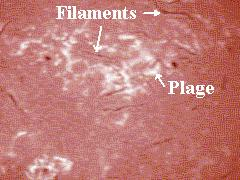
\includegraphics[width=0.5\textwidth]{images/filament.jpg}
	\caption{Filaments. These are images taken in H-alpha. [Image taken from https://solarscience.msfc.nasa.gov/feature2.shtml]}\label{fig:filament} % chktex8
\end{figure}

Since the chromosphere is a relatively understudied part of the chromosphere but still has an important role in space weather, this dissertation will focus on how to model, simulate, and study such a region while at the same time focussing on modern techniques of scientific computing.

%%%%%%%%%%%%%%%%%%%%%%%%%%%%%%%%%%%%%%%%

\chapter{Collisional Plasmas}\label{chap:plasma}

Although plasmas are classically defined as charged gasses, they can coexist with neutral plasma based on the temperature and pressure conditions surrounding them. This means I have two gas mediums, one with the ability to feel Lorentz forces and another that acts like a non-charged fluid. This will generate friction between the fluids when they are moving at different velocities. Due to collision rates being proportional to fluid density and temperature, there can exist a limit in which collision rates are larger than ionization/recombination rates of ions and therefore the fluid becomes collisional. In the reverse case a single-fluid is an apt description as the existence of two-fluids matters largely on the chemistry rather than the collisions. We will be focusing on hydrogen plasmas for our chromosphere case in Chapter~\ref{chap:chromosphere} and in that case two-fluids will be investigated.

\section{Magnetohydrodynamics}\label{sec:mhd}

Magnetohydrodynamics (MHD) is a fluid approximation of plasma popular amongst macroscopic studies of space plasmas. In order to arrive at the fluid approximation I must first look at the particles first and ensure the approximation is appropriate for our case. All of physics is a model and to go from the kinetic theory of plasmas by modeling particles to MHD plasmas by modeling fluids there must be a derivation since there are less assumptions in the kinetic theory than there are in MHD\@.

\subsection{Kinetic Theory}\label{sec:kinetictheory}

We start by assuming an ensemble phase space of particles $f(\textbf{x}, \textbf{v}, t)$ called the distribution function. $\textbf{x}$ is the location of the particle distribution in space, $\textbf{v}$ is the velocity distribution and $t$ is the time. To study the distribution function's evolution through time I take the full derivative with respect to time $\frac{df}{dt}$ which by the product rule turns out to be:

\begin{equation}
	\frac{\partial f}{\partial t} + \frac{\partial \textbf{x}}{\partial t} \cdot \nabla_{\textbf{x}} f + \frac{\partial \textbf{v}}{\partial t} \cdot \nabla_{\textbf{v}} f = {(\frac{\delta f}{\delta t})}_{collisions}
\end{equation}

This is called the Boltzmann equation~\citep{lerner2005}. The term on the right hand side exists due to collisions changed the distribution function in its own way, this also include collisional ionization and other collisional effects that would change the distribution of particles. Simplifying the equation further by substituting how I expect the bulk particles to interact with fields I can get:
 
\begin{equation}
	\frac{\partial f}{\partial t} + \textbf{v} \cdot \nabla_{\textbf{x}} f + \frac{q}{m} (\textbf{E} + \textbf{v} \times \textbf{B}) \cdot \nabla_{\textbf{v}} f = {(\frac{\delta f}{\delta t})}_{collisions}
\end{equation}

Where $q$ is the charge of the particle, $m$ is the mass of the particle, $\textbf{E}$ is the electric field and $\textbf{B}$ is the magnetic field.

This is the kinetic theory of plasmas. The assumptions made here are probability distributions of particles instead of singular particle effects. There are simulations and codes that model particles directly but because of the large memory size of such simulations the region of study must be very small. 

\subsection{Moments of the Distribution}\label{sec:moments}

	In order to arrive at the macroscopic variables I must make an assumption about the distribution of the fluid. This is the most fundamental assumption of MHD is that the distribution of the particles are behaving like a Maxwellian velocity distribution~\citep{mandl1988}. If it is not the case that the velocity distribution is Maxwellian then the approach of MHD is challenged and must be rewritten and integrated differently. The Maxwellian velocity distribution is common in space plasmas that are in thermal equilibrium with itself which lends to the popularity of MHD\@.

\begin{equation}
	f(v) = n {(\frac{m}{2\pi k_B T})}^{3/2} \exp{(-\frac{mv^2}{2k_B T})}
\end{equation}

Where $v = |\textbf{v}|$ is the speed, $k_B$ is the Boltzmann constant and $T$ is temperature. This is assuming a Maxwellian velocity distribution over a thermal equilibrium and a thermal speed.

To arrive at the MHD equations I start to take the `velocity moments' of the equations in order to have macroscopic variables that don't depend on phase speed.

\begin{equation}
	{Moment}_a(\textbf{x}, t) = \int{\textbf{v}^a f(\textbf{x}, \textbf{v}, t)}d\textbf{v}
\end{equation}

Here $a$ is the order of the moment. The first few moments are of interest. The zeroth moment is the continuity equation.

\begin{equation}\label{eq:continuityequation}
	\frac{\partial n_s}{\partial t} + \nabla \cdot (n_s \textbf{v}_s) = {(\frac{\delta n_s}{\delta t})}_{source}
\end{equation}

Each species, $s$, of fluid has its own continuity equations but may be related by the source terms. The source terms come from integrating the collisional ionization, radiative recombination, etc.

The first order moment will give us the momentum equations:

\begin{equation}\label{eq:momentumequation}
	\frac{\partial n_s \textbf{v}_s}{\partial t} + \nabla \cdot (n_s \textbf{v}_s \textbf{v}_s + \frac{\textbf{P}_s}{m_s} ) -n_s \frac{q}{m_s}(\textbf{E} + \textbf{v}_s \times \textbf{B}) = {(\frac{\delta n_s \textbf{v}_s}{\delta t})}_{source}
\end{equation}

Where $\textbf{P}_s$ is the kinetic pressure tensor and can be simplified to the ideal gas law $P_s\textbf{I} = n_s k_B T_s \textbf{I}$ if applicable. The source terms due to the zeroth order also exists here as well as frictional terms that may appear in multi-fluid cases. It is apparent that this equation is fluid-like, a form of the Navier-Stokes equation and hence the naming of these equations as hydrodynamic.

To close the system equations I need one more for the pressure shown previously. So integrating for the second moment gives:

\begin{equation}\label{eq:energyequation}
	\frac{\partial E_s}{\partial t} + \nabla \cdot (\textbf{v}_s E_s) + \nabla \cdot \textbf{q}_s = {(\frac{\delta E_s}{\delta t})}_{source}
\end{equation}

Where $q$ is the heat flow tensor which can be approached in multiple ways and $E$ is the total energy:

\begin{equation}\label{eq:energy}
	E_s = e_s + \frac{1}{2} m_s {v^2}_s + E_{potential}
\end{equation}

Here $e$ is the internal energy and the potential energy is based on the momentum equation's extra acceleration terms like the fields or gravitational potential energy if included.

\subsection{Multi-fluid MHD}\label{sec:multifluidmhd}

In order to make our code capable to solve the equations shown in the previous section (Section~\ref{sec:moments}) further approximations must be done. The three fluids of interest in a hydrogen plasma that includes neutrals are hydrogen ions, electrons and neutral hydrogen. Our plasma is collisional and in partially ionized plasmas I can use the Krook collision term~\citep{bhatnagar1954}.

\begin{equation}\label{eq:krook}
	{(\frac{\delta f}{\delta t})}_{collisions} = \nu_n (f_n - f)
\end{equation}

Where subscript $n$ is the neutral species and $\nu$ is the collision rate. We can find the collision rate simply by using the collision cross-section of neutral particles and the average thermal speed. The average thermal speed is used because temperature in the case of MHD is based on the `peculiar' speeds of the particles (i.e.\ particles with velocity other than that of the bulk plasma). This way peculiar velocities contribute to collisions because if both fluids are moving in the same direction.

\begin{equation}\label{eq:collisionrate}
	\nu_n = n_n \sigma_n <v>
\end{equation}

The thermal speed is a function of temperature and under the Maxwellian velocity distribution assumption, $\sigma$ is the collisional cross-section which can be found in the literature through experiments. The collisional cross-section between ion and electrons include Coulomb effects as well.

The moment equations (Equation~\ref{eq:continuityequation}-\ref{eq:energyequation}) for the three species will look like this:

\begin{equation}\label{eq:icontinuity}
	\frac{\partial n_i}{\partial t} + \nabla \cdot (n_i \textbf{v}_s) = S - L
\end{equation}

\begin{equation}\label{eq:econtinuity}
	\frac{\partial n_e}{\partial t} + \nabla \cdot (n_e \textbf{v}_s) = S - L
\end{equation}

\begin{equation}\label{eq:ncontinuity}
	\frac{\partial n_n}{\partial t} + \nabla \cdot (n_n \textbf{v}_s) = L - S
\end{equation}

\begin{equation}\label{eq:imomentum}
	\begin{aligned}
	& \frac{\partial n_i \textbf{v}_i}{\partial t} + \nabla \cdot (n_i \textbf{v}_i \textbf{v}_i + \frac{\textbf{P}_i}{m_i} ) - n_i \frac{q_i}{m_i}(\textbf{E} + \textbf{v}_i \times \textbf{B}) \\
	& = - \sum_{i \neq s} [n_i \nu_{is}(\textbf{v}_i - \textbf{v}_s)] + \frac{1}{m_i} (S m_n \textbf{v}_n - S m_e \textbf{v}_e -L m_i \textbf{v}_i)
\end{aligned}
\end{equation}

\begin{equation}\label{eq:emomentum}
	\begin{aligned}
	& \frac{\partial n_e \textbf{v}_e}{\partial t} + \nabla \cdot (n_e \textbf{v}_e \textbf{v}_e + \frac{\textbf{P}_e}{m_e} ) - n_e \frac{q_e}{m_e}(\textbf{E} + \textbf{v}_e \times \textbf{B}) \\
	& = - \sum_{e \neq s} [n_e \nu_{es}(\textbf{v}_e - \textbf{v}_s)] + \frac{1}{m_e} (S m_n \textbf{v}_n - S m_i \textbf{v}_i - L m_e \textbf{v}_e)
\end{aligned}
\end{equation}

\begin{equation}\label{eq:nmomentum}
	\begin{aligned}
	& \frac{\partial n_n \textbf{v}_n}{\partial t} + \nabla \cdot (n_n \textbf{v}_n \textbf{v}_n + \frac{\textbf{P}_n}{m_n} ) \\
	& = - \sum_{n \neq s} [n_n \nu_{es}(\textbf{v}_n - \textbf{v}_s)] + \frac{1}{m_n} (L(m_i\textbf{v}_i+m_e\textbf{v}_e) -S m_n \textbf{v}_n)
\end{aligned}
\end{equation}

$S$ and $L$ are source and loss terms respectively due to chemistry processes like ionization and recombination. These are three-fluid MHD equations if the only ion considered is the hydrogen ion.

\subsection{Temperature Equation}

We wish to study the thermal evolution of a plasma in Chapter~\ref{chap:chromosphere}. For this I must transform the energy equation (Equation~\ref{eq:energyequation}) to a form that evolves thermal pressure. We can do this by taking the dot product of the momentum equation and subtracting it from the energy equation. This leaves the energy equation with the thermal energy equation:

\begin{equation}\label{eq:pressureequation}
	\frac{\partial }{\partial t}\frac{P_s}{\gamma_s - 1} +\nabla\cdot(\frac{P_s}{\gamma_s -1}\textbf{v}_s) + (1 - \frac{P_s}{\gamma_s - 1}) \nabla\cdot\textbf{v}_s = {(\frac{\delta E_s}{\delta t})}_{source} - \textbf{v}_s \cdot(\frac{\delta m_s n_s\textbf{v}_s}{\delta t})
\end{equation}

Elastic collisions may take the form of~\citep{Banks1973}:

\begin{equation}\label{eq:energycollisions}
	{(\frac{\delta E_s}{\delta t})}_{collisions} = \textbf{v}_s \cdot {(\frac{\delta m_s n_s \textbf{v}_s}{\delta t})}_{collisions} + m_{sn} \nu_{sn} n_s [ (3 k_B / m_s) (T_n - T_s) + \lvert \textbf{v}_s - \textbf{v}_n \rvert^2 ]
\end{equation}

Where $m_{sn}$ is the reduced mass of the species with the neutral species, $T$ is temperature, $k_B$ is the Boltzmann constant. The previous equation shows thermal exchange due to collision between the species as well as {\it frictional heating\/} term that is proportional to the difference in speeds between the two. For a conservative scheme it is more approriate to use the total energy equation, but this depends on a case by case basis. The CoMFi code is capable of doing both approaches. For the chromosphere I will be concerned with the thermal evolution.

\subsection{Two-fluid MHD}\label{sec:2fluidmhd}

The ion and electron fluid can be simplified further to be one plasma that tracks the center of momentum between the two. Plasmas are typically quasi-neutral, it has as many positive charges as negative ones. Any imbalance in the charge will create a strong electric field within the plasma and strongly attract outside sources of charges until it is quasi-neutral again. In single hydrogen ion case that means:


\begin{equation}\label{eq:quasineutrality}
	n_i = n_e = n
\end{equation}

This can simplify the current density equation as well:

\begin{equation}\label{eq:currentdensity}
	\textbf{J} = e ( n_i \textbf{v}_i - n_e \textbf{v}_e) = e n (\textbf{v}_i - \textbf{v}_e)
\end{equation}

Where $e$ is the elementary charge. Subtracting the ion and electron continuity equations gives:
\begin{equation}
	\frac{\partial n_i - n_e}{\partial t} + \nabla\cdot(n_i v_i - n_e v_e) = 0
\end{equation}
The charge conservation equation.
\begin{equation}\label{eq:chargeconservation}
	\nabla\cdot\textbf{J} = 0
\end{equation}


To simplify the three MHD equations (Equations~\ref{eq:imomentum}-\ref{eq:nmomentum}) I can take the multiple of their masses and add Equation~\ref{eq:imomentum} and~\ref{eq:emomentum}.

\begin{equation}\label{eq:singlemomentum}
	\begin{aligned}
		& \frac{\partial \rho_i \textbf{v}_i + \rho_e \textbf{v}_e}{\partial t} + \nabla \cdot (\rho_e \textbf{v}_e \textbf{v}_e + \rho_i \textbf{v}_i \textbf{v}_i + \textbf{P}_i + \textbf{P}_e) - \textbf{J} \times \textbf{B} \\
		& = - \rho_i \nu_{in}(\textbf{v}_i - \textbf{v}_n) - \rho_e \nu_{en} (\textbf{v}_e - \textbf{v}_n)+ (S m_n \textbf{v}_n - L m_i \textbf{v}_i - L m_e \textbf{v}_e)
\end{aligned}
\end{equation}

The $\rho$ here is the mass density of the fluid. Using the induction equation Maxwell's equations I can simplify $\textbf{J} \times \textbf{B}$ further.

\begin{equation}
	\textbf{J} \times \textbf{B} = \frac{1}{\mu_0} (\nabla \times \textbf{B}) \times \textbf{B} = -\nabla \cdot (\frac{B^2}{2\mu_0}\textbf{I} - \textbf{BB})
\end{equation}

This way I can have a magnetic flux and make use of our conservative scheme in Section~\ref{sec:tvd-muscl}. Finally by dividing by $m_i+m_e$ to Equation~\ref{eq:singlemomentum} I can find the center of momentum velocity and simplify the equation one last time:

\begin{equation}
	\textbf{V} = \frac{\rho_i \textbf{v}_i + \rho_e \textbf{v}_e}{\rho_i+\rho_e}
\end{equation}

\begin{equation}\label{eq:vi}
	\textbf{v}_i = \textbf{V} + \frac{\rho_e}{\rho_i+\rho_e} \frac{1}{n e} \textbf{J} \sim \textbf{V} + \frac{m_e}{m_i} \frac{\textbf{J}}{n e} 
\end{equation}

\begin{equation}\label{eq:ve}
	\textbf{v}_e = \textbf{V} - \frac{\rho_i}{\rho_i+\rho_e} \frac{1}{n e} \textbf{J} \sim \textbf{V} -\frac{\textbf{J} }{n e}
\end{equation}

\begin{equation}\label{eq:momentumcom}
\begin{aligned}
	&\frac{\partial \rho \textbf{V}}{\partial t} + \nabla \cdot (\textbf{K}_{i,e} + \frac{B^2}{2\mu_0}\textbf{I} - \frac{\textbf{BB}}{\mu_0}) \\
	&= - (\rho_i \nu_{in} + \rho_e \nu_{en})(\textbf{V} - \textbf{U}) + \frac{m_e}{e}(\nu_{en}-\nu_{in}) \textbf{J} \\
	& + [S m_n \textbf{U} - L m_i (\textbf{V} + \frac{m_e}{m_i} \frac{\textbf{J}}{n e})- L m_e (\textbf{V} -\frac{\textbf{J}}{n e})]
\end{aligned}
\end{equation}

The dynamic pressure and thermal pressures have been combined into one kinetic tensor term $\textbf{K}$. $\textbf{U}$ is the neutral velocity.

The neutral momentum equation is much easier since it is not affected by the Lorentz force and the momentum exchange is reversed, so it becomes:

\begin{equation}\label{eq:momentumneutral}
\begin{aligned}
	&\frac{\partial \rho_n \textbf{U}}{\partial t} + \nabla \cdot (\textbf{K}_n) \\
	&= (\rho_i \nu_{in} + \rho_e \nu_{en})(\textbf{V} - \textbf{U}) - \frac{m_e}{e}(\nu_{en}-\nu_{in}) \textbf{J} \\
	& - [S m_n \textbf{U} - L m_i (\textbf{V} + \frac{m_e}{m_i} \frac{\textbf{J}}{n e})- L m_e (\textbf{V} -\frac{\textbf{J}}{n e})]
\end{aligned}
\end{equation}

Finally, following the ideal gas law $P_s = n_s k_B T_s$ and the monoatomic ratio of specific heats $\gamma = 5/3$, the last two equations needed are the temperature equations of the two fluids:

\begin{equation}\label{eq:temperatureion}
	\begin{aligned}
		&\frac{3}{2} n [\frac{\partial k_B T}{\partial t} + \nabla\cdot(k_B T \textbf{V})] - \frac{1}{2} n k_B T (\nabla\cdot\textbf{V}) + \nabla\cdot\textbf{q} \\
	& = n m_{in} \nu_{in} [ 3 k_B (T_n - T) + m_n \lvert \textbf{U} - \textbf{V} \rvert^2 ] + Q
	\end{aligned}
\end{equation}

\begin{equation}\label{eq:temperatureneutral}
	\begin{aligned}
		&\frac{3}{2} n_n [\frac{\partial k_B T_n}{\partial t} + \nabla\cdot(k_B T_n \textbf{U})] - \frac{1}{2} n_n k_B T_n (\nabla\cdot\textbf{U}) + \nabla\cdot\textbf{q} \\
	&= n_n m_{ni} \nu_{ni} [ 3 k_B (T - T_n) + m_i \lvert \textbf{V} - \textbf{U} \rvert^2 ] + Q_n
	\end{aligned}
\end{equation}

Where $\textbf{q}$ is the heat flux and $Q$ are other heating and cooling terms such as radiative losses.


\section{Maxwell's Equations}

Since a plasma is a gas the reacts strongly to electro-magnetic fields. Maxwell's equations must be enforced in order to have a plasma consistent with reality. The Maxwell equations will also help us with the time evolution of the fields, as the fields are interconnected. The Maxwell's equations are:

\begin{equation}\label{eq:gausslaw}
	\varepsilon_0\nabla\cdot\textbf{E} = n q
\end{equation}
\begin{equation}\label{eq:maggausslaw}
	\nabla\cdot\textbf{B} = 0
\end{equation}
\begin{equation}\label{eq:lawofinduction}
	\frac{\partial\textbf{B}}{\partial t} = - \nabla\times\textbf{E}
\end{equation}
\begin{equation}\label{eq:ampereslaw}
	\mu_0\varepsilon_0\frac{\partial\textbf{E}}{\partial t} + \mu_0\textbf{J} = \nabla\times\textbf{B}
\end{equation}

In a plasma, any evolution of the electric field is very quickly resolved in the timescales I am considering. Ions and electrons would rearrange quickly to cancel out the electric field so it can be assumed as a perfect electrical conductor. This means the evolution of the magnetic field is more useful than the evolution of the electric field in timescales of interest. This also leads to the approximation $\partial\textbf{E}/\partial t \sim 0$:

\begin{equation}\label{eq:ampereslawapprox}
	\mu_0\textbf{J} = \nabla\times\textbf{B}
\end{equation}

The plasma is therefore in a static electric field. We will need a definition of the electric field in order to evolve our magnetic fields. This will be discussed in the next Section~\ref{sec:ohmslaw}.

The magnetic field has also never been observed to have monopoles which makes it a solenoidal vector field. This is called Gauss's law of magnetism. The magnetic field will need to keep this shape despite errors in the simulation. The implementation will be discussed in Section~\ref{sec:divergencefree}.

\subsection{Generalized Ohm's Law}\label{sec:ohmslaw}

When talking about the Generalized Ohm's Law (GOL) or the Ohm's Law we typically think about conductivity in metal. Or at least that is how it is taught in college level physics. The Generalized Ohm's Law's purpose is to find the electric field within the plasma. This can be found by subtracting the ion and electron momentum equations~\ref{eq:imomentum}-\ref{eq:emomentum} and multiplying by electron mass.

\begin{equation}
\begin{aligned}
	&\frac{m_e}{e}\frac{\partial \textbf{J}}{\partial t} + \nabla \cdot (m_e n [\textbf{v}_i \textbf{v}_i - \textbf{v}_e \textbf{v}_e] +m_e \frac{\textbf{P}_i}{m_i} - \textbf{P}_e) - n e (-\frac{m_e}{m_i}+1) \textbf{E} - \frac{n e m_e}{m_i} \textbf{v}_i \times \textbf{B} - n e\textbf{v}_e \times \textbf{B} \\
	&= -n m_e [ \nu_{ie} (\textbf{v}_i -\textbf{v}_e) + \nu_{in} (\textbf{v}_i -\textbf{v}_n) - \nu_{ei} (\textbf{v}_e -\textbf{v}_i) - \nu_{en} (\textbf{v}_e -\textbf{v}_n)] \\
	&+ (\frac{m_e}{m_i} - 1) S m_n \textbf{v}_n - \frac{m_e}{m_i} S m_e \textbf{v}_e - L m_e \textbf{v}_i + S m_n \textbf{v}_n - S m_i \textbf{v}_i - L m_e \textbf{v}_e
\end{aligned}
\end{equation}

Simplifying further by taking the $m_e/m_i \sim 0$ approximation, current density~\ref{eq:currentdensity}, charge conservation~\ref{eq:chargeconservation}, and the velocity definitions~\ref{eq:vi} and~\ref{eq:ve}.

\begin{equation}
\begin{aligned}
	&\frac{m_e}{n e^2} \frac{\partial\textbf{J}}{\partial t}+ \frac{m_e}{ne^2} \nabla\cdot[\textbf{V}\textbf{J} + \textbf{J}\textbf{V}] + \frac{-\nabla\cdot\textbf{P}_e + \textbf{J}\times\textbf{B}}{ne}- \textbf{E} - \textbf{V}\times\textbf{B} \\
	& = - \frac{m_e}{e}[\nu_{in} (\textbf{V}-\textbf{v}_n) + \nu_{en}(\textbf{V} - \textbf{v}_n)] - \eta\textbf{J}
\end{aligned}
\end{equation}
\begin{equation}\label{eq:gom}
\begin{aligned}
	&\textbf{E}  = - \textbf{V}\times\textbf{B} + \frac{m_e}{n e^2} \frac{\partial\textbf{J}}{\partial t}+ \frac{m_e}{ne^2} \nabla\cdot[\textbf{V}\textbf{J} + \textbf{J}\textbf{V}] \\
	&+ \frac{-\nabla\cdot\textbf{P}_e + \textbf{J}\times\textbf{B}}{ne} \\
	&  + \frac{m_e}{e}[\nu_{in} (\textbf{V}-\textbf{U}) - \nu_{en}(\textbf{V} - \textbf{U})] + \eta\textbf{J}
\end{aligned}
\end{equation}


Where $\eta = \frac{m_e \nu_e}{e^2 n}$ is the Ohmic resistivity. The relation between the electric field and the resistivity is what we think of when we invoke Ohm's law in college physics. Clearly the equation is a little more complicated in MHD\@. Note that collision with neutrals may change the electric field also. The collisions can cause a drift between the ions and electrons, separating them and causing an electric field.

We can take Equation~\ref{eq:gom} a step further and eliminate the need for an evolving current and instead use the low-frequency approximation (i.e.\ the time scales is much smaller than the plasma frequency $\omega_p = \sqrt{\frac{n_e e^2}{\varepsilon_0 m_e}}$). Removing the convective derivate of the current gives this approximation:

\begin{equation}\label{eq:gomlowfreq}
\begin{aligned}
	&\textbf{E}  = - \textbf{V}\times\textbf{B} \\
	&+ \frac{-\nabla\cdot\textbf{P}_e + \textbf{J}\times\textbf{B}}{ne} \\
	&  + \frac{m_e}{e}[\nu_{in} (\textbf{V}-\textbf{U}) - \nu_{en}(\textbf{V} - \textbf{U})] + \eta\textbf{J}
\end{aligned}
\end{equation}

And in a two-fluid approach I may define current along with the same assumptions:
\begin{equation}
	\textbf{J} = \frac{\nabla\times\textbf{B}}{\mu_0}
\end{equation}

The collisional terms may also be ignored under careful consideration of how small $\frac{\nu}{\omega^2_p}$ may be.

In Chapter~\ref{chap:chromosphere} I will simplify the above equation further to suit our needs. Typically in simulations you only want to include the terms that matter the most. With careful consideration I can come up with a GOL that is most appropriate for our application.

\subsection{Induction Equation}

To close our set of equations I need a way to evolve the magnetic fields. For this I can use the law of induction (Equation~\ref{eq:lawofinduction}) with the GOL (Equation~\ref{eq:gomlowfreq}).

\begin{equation}
	\begin{aligned}
		\frac{\partial\textbf{B}}{\partial t} =& \nabla\times(\textbf{V}\times\textbf{B} - \frac{-\nabla\cdot\textbf{P}_e + \textbf{J}\times\textbf{B}}{ne} \\
						       &- \frac{m_e}{e}[\nu_{in} (\textbf{V}-\textbf{U}) - \nu_{en}(\textbf{V} - \textbf{U})] - \eta\textbf{J})
\end{aligned}
\end{equation}

We may use vector identities to transform the advective terms.

\begin{equation}
	\nabla\times(\textbf{V}\times\textbf{B}) = \nabla\cdot(\textbf{BV}-\textbf{VB})
\end{equation}

This also gives the opportunity to have as many terms in conservative forms as I can.
\begin{equation}\label{eq:inductionequation}
	\begin{aligned}
		& \frac{\partial\textbf{B}}{\partial t} = \\
		&\nabla\cdot(\textbf{BV}-\textbf{VB} + \textbf{B}\textbf{V}_{hall}-\textbf{V}_{hall}\textbf{B}) \\
		&-k_B (\frac{\nabla n \times \nabla T_e}{ne}) \\
		&- \nabla\times(\frac{m_e}{e}[\nu_{in} (\textbf{V}-\textbf{U}) - \nu_{en}(\textbf{V} - \textbf{U})]) \\
		& - \frac{1}{\mu_0} \nabla\eta\times\textbf{J} + \eta\nabla^2\textbf{B}
\end{aligned}
\end{equation}

Where

\begin{equation}
	\textbf{V}_{hall} = \frac{\textbf{J}}{ne}
\end{equation}

Since it is associated with the Hall term in the induction equation.

In the coming chapters I will be using a simplified form of the GOL---dropping the terms that are less significant.

\chapter{Implementation}\label{chap:implementation}

Computational fluid dynamics is a well studied field in computer science, numerics and engineering. Many of its principles can be applied to MHD due to the fluid nature of its equations. We will be focusing on only the ones implemented in the code my for this dissertation, the Collisional Multi-Fluid ion (CoMFi) code made for the chromosphere case which will be explored in more detail in the upcoming chapter (Chapter~\ref{chap:chromosphere}). The code is an ever-evolving code that uses Graphical Processing Units (GPUs) instead of the common CPUs you see for MHD codes. This is to implement MHD that makes use of the frontiers of computer technology. GPUs were made for graphical operations in video games. This means they are specifically designed to be very fast at matrix rotations, translations and other linear algebra. In this chapter I will explore proper general purpose GPU programming techniques for solving differential equations and the schemes used alongside it. CoMFi is written in C++ using ViennaCL for GPU linear algebra template programming and Armadillo for setting up the matrices on the CPU (the reason for this will be discussed in).

\section{Schemes}\label{sec:schemes}

CoMFi uses the conservative MHD equations therefore conservative schemes are of interest. This makes use of the conservative variables unknowns as opposed to the primitive variables ($n v$ as opposed to $v$). This way I can use a finite-volume-method and conserve these quantities to the machine rounding error. Conservative schemes are also known to do well at capturing shocks and the chromosphere is a region where I expect such shocks to exist.

\begin{equation}\label{eq:geneuler}
	\frac{\partial \textbf{u}}{\partial t} + \nabla \cdot \textbf{F(u)} = 0
\end{equation}

The above equation is a general Euler equation demonstrating a conservation law problem. The quantity to be conserved is $\textbf{u}$ and is a function the flux $\textbf{F}$. We will be considering the linear case for simplicity however MHD has demonstrably non-linear terms as the flux (e.g. Equation~\ref{eq:imomentum}) but it can easily follow from this linear case. The point is to show the total volume is conserved:

\begin{equation}\label{eq:geneulerint}
	\frac{d\textbf{u}}{dt} + \frac{1}{V} \oint \textbf{F} \cdot \textbf{n} dS
\end{equation}

In codes designed to solve differential equations numerically I must decide on the discretization. Since I am using a finite-volume-method I am discretizing the domain by cells with density quantities in them. The code is discretized in cells existing in Cartesian coordinates (rectangular cells) so I am tasked to find the values of the variables at the cell faces in order to conserve the volume.

We would also like a total-variation-diminishing (TVD) scheme, this is because spatial derivatives are approximated on a computer. If I take a Taylor series of a derivative from one cell to another and compare with an approximate derivative like $\frac{u(x+\Delta x)-u(x-\Delta x)}{2\Delta x}$ I see that there are many higher order terms missing. Taking the Fourier analysis of these terms show that any high-frequency errors may compound (sometimes referred to as spurious oscillations). This can be fixed by schemes that ensure the total variation $TV$ is diminishing.

\begin{equation}\label{eq:tvd}
	\frac{d(TV)}{dt} = \frac{d}{dt} \int \lvert \frac{\partial u}{\partial x} \rvert dx \leq 1
\end{equation}

Therefore, for the purpose of our code, I will use the Total-Variation-Diminishing Monotonic Upwind Scheme for Conservation Laws (TVD-MUSCL).

\subsection{Flux Limiters}\label{sec:fluxlimiters}

To conserve the cell's quantities I must be able to approximate the quantities on the cell edges. At the same time I must preserve monotonicity to avoid the oscillations. This can be achieved through flux limiters. The utility of the flux limiters is to turn the scheme into a first-order upwind scheme in sharp discontinuities and a high-resolution scheme when the solution is smooth.

\begin{equation}\label{eq:fluxlimiter}
	u_{j+1/2} = u_j + \frac{1}{2} \phi(r_j) (u_{j+1} - u_j)
\end{equation}
\begin{equation}
	r_j = \frac{u_j - u_{j-1}}{u_{j+1} - u_j}
\end{equation}

Subscript $j$ is the discretized cell location with quantity $u$. The ratio of successive gradients $r$ determines how strongly the flux limiter acts to find the extrapolated cell edge variable. The flux limiter $\phi$ includes the cells around edge more readily the smoother the solution is ($r>0$), or sharp it is ($r<0$) in which case the flux limiter is zero ($\phi=0$). These are the properties flux limiters must abide in order to turn the scheme upwind in sharp gradients or high-resolution in smoother gradients. The above equation is a linear reconstruction of a cell edge. Other reconstructions exist but are more diffusive and avoids the shock-capturing goal of the code.

We have some freedom in choosing how to set the flux limiter. Many flux limiters have been made and studied in the past. The simplest flux-limiter is the minmod.

\begin{equation}\label{eq:minmod}
	\phi_{minmod}(r) = \max(0, \min(1, r)), \lim_{r \to \infty} \phi(r) = 1
\end{equation}

The CoMFi code provides several flux limiters (see Appendix~\ref{app:fluxlimiters}) and finding the best one is a matter of trial and error. The limiter used by default is the van Albada limiter.

\begin{equation}\label{eq:vanalbada}
	\phi_{va}(r) = \frac{r^2 + r}{r^2 + 1}, \lim_{r \to \infty} \phi(r) = 1
\end{equation}

Implementing these on a computer however is not a trivial task. Many initial conditions require the entirety of the domain be the same number for instance. In that case I get an $r = \frac{0}{0}$ and this causes a computer to return NaN (not a number). Setting to $r=0$ is appropriate but requires extra coding. A work around is to add a small number $\epsilon$ to the denominator known as the machine epsilon to avoid these cases.

\begin{equation}
	r_j = \frac{u_j - u_{j-1}}{u_{j+1} - u_j + \epsilon}
\end{equation}

This machine epsilon should have no effect on the result so long as the variables have been normalized appropriately (see Section~\ref{sec:normalization}). This means the valuable results are within an order of magnitude so the machine epsilon of a 64bit floating point number of $2^{-−52} \sim 2.22 \times 10^{-16}$ would be negligible. If two adjacent cells have the same value, as is common with initial values, then dividing by zero is usefully avoided.

\subsection{TVD-MUSCL}\label{sec:tvd-muscl}

The TVD-MUSCL scheme reconstructs `left' ($L$) and `right' ($R$) states of the cell edge variables. 

\begin{equation}
	u^L_{j-1/2} = u_{j-1} + \frac{1}{2} \phi(r_{j-1}) (u_j - u_{j-1})
\end{equation}
\begin{equation}
	u^L_{j+1/2} = u_{j} + \frac{1}{2} \phi(r_{j}) (u_j - u_{j-1})
\end{equation}
\begin{equation}
	u^R_{j-1/2} = u_{j} + \frac{1}{2} \phi(r_{j}) (u_{j+1} - u_{j})
\end{equation}
\begin{equation}
	u^R_{j+1/2} = u_{j+1} + \frac{1}{2} \phi(r_{j+1}) (u_{j+1} - u_{j})
\end{equation}

With the left and right extrapolated variables I may construct a flux.

\begin{equation}
	F^*_{j-1/2} = \frac{1}{2} ([F(u^R_{j-1/2})+F(u^L_{j-1/2})] - \lambda_{j-1/2}[u^R_{j-1/2}-u^L_{j-1/2}])
\end{equation}
\begin{equation}
	F^*_{j+1/2} = \frac{1}{2} ([F(u^r_{j+1/2})+F(u^l_{j+1/2})] - \lambda_{j+1/2}[u^r_{j+1/2}-u^l_{j+1/2}])
\end{equation}

Here $F u = \lambda u$ are the eigenvalues of the variables. This in physical terms means the largest wave speeds of the system. Typically for the ion plasma it is the fast-mode speed and for the neutrals it is the sound speed. It's important to note in conservative MHD this is only the wave speed ($c_{fast}$) and not the same as the fastest speed of information propagation ($v+c_{fast}$). The diffusive terms proportional to $\lambda$ are meant to avoid the oscillations and if they are larger than they need to be the solution will be more diffusive.


\section{Enforcing a Solenoidal Magnetic Field}\label{sec:divergencefree}

The Gauss's law for magnetic fields (Equation~\ref{eq:maggausslaw}) needs to be taken care of because due to machine rounding error and other errors due to discretization, there will be evolution of the divergence. That is to say, although:
\begin{equation}
	\frac{\partial\nabla\cdot\textbf{B}}{\partial t} = -\nabla\cdot\nabla\times\textbf{E} = 0
\end{equation}

The reality is, due to errors:
\begin{equation}
	\frac{\partial\nabla\cdot\textbf{B}}{\partial t} = \epsilon_{errors}
\end{equation}

There are many methods to resolving this. A popular method is Yee grids, sometimes referred to as staggered grids. Placing the magnetic fields to the cell edges of the electric fields. By doing this, evolving the magnetic fields reduces errors to machine rounding errors since Stokes' theorem is imposed on the problem.

\begin{equation}\label{eq:stokesyee}
	\iint_S\frac{\partial\textbf{B}}{\partial t}\cdot d\textbf{A} = {\oint}_{edges} \textbf{E}\cdot d\textbf{l}
\end{equation}

This is not the method used for CoMFi. Staggering the grid makes using a finite-volume-method difficult especially when trying to find cell centers from one quantity to the next. Instead I employ the Generalized Lagrange Multiplier method introduced by~\citet{glm}.

\subsection{Generalized Lagrange Multiplier}

The Generalized Lagrange Multiplier (GLM) method adds another unknown to the system of equations to be solved. This has the drawback of using more memory. Its implementation is simple, however, which means adding it to an existing code is easy. The GLM $\Phi$ tries to minimize the monopoles created due to errors in the simulation. It does this by first creating some stress to the induction equation if there is some monopole.

\begin{equation}
	\frac{\partial\textbf{B}}{\partial t} = - \nabla\times\textbf{E} + \nabla \Phi
\end{equation}

And filter the monopoles into the GLM using this method of evolution:
\begin{equation}
	\mathcal{D}(\Phi) + \nabla\cdot\textbf{B} = 0
\end{equation}

$\mathcal{D}$ is a differential operator and I can choose the GLM to evolve in any way I want. A hyperbolic evolution and/or a parabolic evolution may be used. Due to the non-linear and parabolic nature of our equations I opt to use both:

\begin{equation}
	\matchal{D}(\Phi) = \frac{1}{c^2_h}\frac{\partial\Phi}{\partial t} + \frac{1}{c^2_p}\Phi
\end{equation}

Here $c_h$ and $c_p$ are the hyperbolic and parabolic speeds of the divergence errors. That means the divergence errors will propagate at a speed of $c_h$ and dissipate at rate of $c_p$. The new equation that must be solved is:

\begin{equation}\label{eq:glm}
	\frac{\partial\Phi}{\partial t} + c^2_h \nabla\cdot\textbf{B} = - \frac{c^2_h}{c^2_p} \Phi
\end{equation}

The hyperbolic speed, $c_h$, can be chosen to be similar the wave speeds in the magnetic field (i.e.\ the fast-mode speed). We have more freedom to chose the ratio of dissipation to propagation, $\alpha = c_h / c^2_p$, also known as the damping parameter. Through testing 0.5 was find to be a good parameter~\citep[p. 5899-5911]{glm2}.

We can separate Equation~\ref{eq:glm} into two parts two solve. We can solve the right hand side exactly, and use the conservative scheme to solve the second term on the left hand side. First solve the left hand side and setting the right hand side equal to zero. Then minimize it with the exact solution:

\begin{equation}
	\Phi(t+\Delta t) = \Phi(t) e^{-c_h\alpha\Delta t}
\end{equation}

The efficacy of this method is keeping the normalized divergence errors to lower than the normalized grid-spacing. This is useful so that the monopoles are not evident when drawing the magnetic field lines nor does it have a strong effect on the results.

\section{Time Integration}\label{sec:timeintegration}

Time integration is important to the time stepping nature of simulations. We can have both implicit time stepping and explicit time stepping. Explicit time stepping for the Euler equation takes the form:

\begin{equation}\label{eq:explicit}
	u^{n+1} = u^n + v\int^{n+1}_n \frac{d}{dx}(u^{n}) dt
\end{equation}

This is the easiest approach to the solutions because you use values in the previous time step to solve for the next. This does not require a solution of a linear system which I will show later. Explicit schemes are limited to time steps that are smaller than the wave period, $\Delta x / v > \Delta t$, and depending on the scheme a multiple smaller but usually within the same order of magnitude. This is because the largest characteristic speed (the speed of information propagation) cannot be faster than the grid spacing and time steps. This will cause loss of information and instabilities as there will be an attempt to skip grids but due to discretization it will fail to resolve.

In implicit time steps
\begin{equation}\label{eq:implicit}
	u^{n+1} - v\int^{n+1}_n \frac{d}{dx}(u^{n+1}) dt = u^n 
\end{equation}
This introduces a linear equation that must be solved, $Au^{n+1} = u^n$, and the solution is to invert the matrix A, $u^{n+1} = A^{-1} u^n$. This gets more complicated in non-linear systems. In this case I am not limited by that characteristic speed.

There is also a third option, semi-implicit schemes. This integrates some variables implicitly and others explicitly. This is helpful when you do not want to be limited by certain characteristic speeds. For the chromosphere example in Chapter~\ref{chap:chromosphere} a characteristic I try to overcome is the collision times since it is orders of magnitude larger than the Alf\'ven and sound times in the chromosphere.

\subsection{Stability}\label{sec:stability}

In order for schemes to be stable, errors must not grow over time. We can make sure errors are not growing by employing the Von Neumann analysis. Let's use a simple explicit forward difference scheme on the wave equation for example.

\begin{equation}
	\frac{\partial u}{\partial t} = -v\frac{\partial u}{\partial x}
\end{equation}
\begin{equation}\label{eq:upwind}
	u^{n+1}_j = u^n_j - \frac{\Delta t}{\Delta x}v(u^n_{j+1}-u^n_{j})
\end{equation}

The above is the Euler equation for a wave propagating at constant speed $v$ using a forward difference method, also called an upwind scheme. The Von Neumann method takes a Fourier analysis to the error waves generated due to discretization. We say that by using the Taylor series the discretization should have this {\it exact\/} solution.

\begin{equation}
	u_{j+1} = u_j + \Delta x {\frac{\partial u}{\partial x}}\rvert_j + \frac{\Delta x^2}{2} {\frac{\partial^2 u}{\partial x^2}}\rvert_j + \frac{\Delta x^3}{3!} {\frac{\partial^3 u}{\partial x^3}}\rvert_j + \cdots 
\end{equation}

Where $j$ is the location of the cell solution. Rearranging so that it looks like a forward difference scheme shows its relation to the exact solution of the partial derivative.

\begin{equation}
	\epsilon = \frac{u_{j+1} - u_j}{\Delta x} - {\frac{\partial u}{\partial x}}\rvert_j =  \frac{\Delta x}{2} {\frac{\partial^2 u}{\partial x^2}}\rvert_j + \frac{\Delta x^2}{3!} {\frac{\partial^3 u}{\partial x^3}}\rvert_j + \cdots = O(\Delta x)
\end{equation}

This means the errors, $\epsilon$, are of first order, proportional to $\Delta x$ so the upwind scheme is a first order scheme in space. To see how the errors evolve in time I employ the Von Neumman analysis. Assuming the computed solution is a linear combination of the real solution and the error.

\begin{equation}
	u_{computed} = u_{exact} + \epsilon
\end{equation}

We can subtract the exact solution and do a Fourier analysis of the errors found. Doing this on Equation~\ref{eq:upwind} yields.

\begin{equation}
	e^{a(t+\Delta t)+ikx} = e^{at+ikx} - \beta (e^{at + ik(x+\Delta x)}-e^{at + ikx})
\end{equation}

Where $\beta = v(\Delta t / \Delta x)$, $a$ is the component of the errors in time, and $k$ is the series of frequencies of the errors in space. To find the error growth due to time I must find the ratio $e^{at} = u^{n+1}/u^n$.

\begin{equation}
	G = e^{a\Delta t} = 1 - \beta (e^{ik\Delta x}- 1)
\end{equation}

$G$ is the growth in error each time step also called the amplification factor. In order to keep the errors bounded I need to ensure that this ratio is less than or equal to 1.

\begin{equation}
	\lvert G \rvert \leq 1
\end{equation}

For the upwind scheme example I used: 

\begin{equation}
	\lvert 1 - \beta (e^{ik\Delta x}- 1) \rvert \leq 1
\end{equation}

This will lead to

\begin{equation}
	\beta \leq 1
\end{equation}

Or the stability requirement, also known as the Courant-Friedrich-Lewy condition:

\begin{equation}
	v \frac{\Delta t}{\Delta x} \leq 1
\end{equation}

An explicit central difference scheme behaves differently, however.
\begin{equation}\label{eq:central}
	u^{n+1}_j = u^n_j - \beta \frac{u^n_{j+1}-u^n_{j-1}}{2}
\end{equation}

Doing the Von Neumann analysis here using a more simplified notation:
\begin{equation}
	u^{n+1} e^{ijk} = u^n e^{ijk} - \beta \frac{u^n e^{i(j+1)k} - u^n e^{i(j-1)k}}{2}
\end{equation}
\begin{equation}
	G = 1 - \beta \frac{e^{ik} - e^{-ik}}{2} = 1 - i\beta \sin{(k)}
\end{equation}
\begin{equation}
	\lvert 1 - i\beta \sin{(k)} \rvert = 1 + \beta^2 \sin^2(k) \nleq 1
\end{equation}

Since the amplification factor is always larger than 1, errors will always grow. This scheme is {\it unconditionally unstable}. Doing this scheme in an implicit fashion can fix this problem.

\begin{equation}\label{eq:implicitcentral}
	u^{n+1}_j = u^n_j - \beta \frac{u^{n+1}_{j+1}-u^{n+1}_{j-1}}{2}
\end{equation}

Now doing the Fourier analysis,

\begin{equation}
	u^{n+1}_j - \beta \frac{u^{n+1}_{j+1}-u^{n+1}_{j-1}}{2} = u^n_j
\end{equation}
\begin{equation}
	u^{n+1}e^{ijk} - \beta \frac{u^{n+1}e^{i(j+1)k}-u^{n+1}e^{i(j-1)k}}{2} = u^n
\end{equation}
\begin{equation}
	G (1 - \beta \frac{e^{ik}-e^{-ik}}{2}) = 1
\end{equation}
\begin{equation}
	G  = \frac{1}{1 - i \beta \sin{(k)}} 
\end{equation}
\begin{equation}
\lvert G \rvert = \frac{1}{1+\beta^2 \sin^2{(k)}} \leq 1
\end{equation}

Since the amplification factor is always less than or equal to 1 this implicit central difference scheme is {\it unconditionally stable}.

\section{Architecture}\label{sec:architecture}

It is important in scientific computing not to reinvent the wheel. There are many libraries, particularly C++ libraries, that use template programming to make it easier to write linear algebra in code. It is always easier to add an entire vector with one + sign than looping through each element of the two vectors and adding each. For this reason I can avoid low-level programming like Fortran for CPUs or OpenCL and CUDA for GPUs because the Basic Linear Algebra Subroutines (BLAS) have already been written and abstracted by someone else. C++ is a language that is all about abstraction and speed. There is a pervasive myth that if you want to do scientific computing you must use Fortran or CUDA but this is not true and is usually reinforced by scientists' lack of understanding of computer science and/or bad code.

The code uses to template expression libraries in C++. Template expression is how C++ abstracts operators such as $+$, $-$ and $/$ to deal with one variable and the next and call the low level BLAS functions. The libraries used are Armadillo for CPU\@. This is a code typically used for Machine Learning applications so speed and big data is its focus. For GPU programming ViennaCL is used, it's a library used by PETSc for its GPU portion. However, at the time of this writing, PETSc's GPU code is not fully developed so ViennaCL is used directly. Luckily, ViennaCL interfaces with Armadillo well and there exists copy constructors to go from shared memory to GPU memory.

Matrices {\it must\/} be built on the CPU\@. Accessing GPU elements individually is a slow process that is limited by the PCI-e speed and when the machine code (running on CPU) is asked to go back and forth, I get slow code. Best practice is to first build a matrix on the CPU then copy to the GPU\@.

\subsection{Data Structure}\label{sec:datastructure}

When using the semi-implicit method a linear system $Ab^{n+1}=b$ must be solved. We must think of an appropriate ordering of our vector in terms of the where the unknowns must be in the elements of the vector. For GPU programming in order to take advantage of its matrix operations speeds due to its many cores I must also be easily able to change back and forth between matrix and vector form between the implicit and explicit portions of the solution. A good ordering for a two-dimensional domain looks like this:

\begin{equation}
	b =
\begin{bmatrix}
	u_{0,00} \\
	\vdots \\
	u_{0,i0} \\
	\vdots \\
	u_{0,ij} \\
	\vdots \\
	u_{w,ij} \\
\end{bmatrix}
\end{equation}

The subscripts $i$ and $j$ describe the location of the cell in the $x$ and $y$ axis respectively and $w$ are the scalar unknowns.

\begin{equation}
	u_w = 
	\begin{bmatrix}
		B_x \\
		B_{\perp} \\
		B_z \\
		n_i \\
		n_n \\
		n_i V_x \\
		n_i V_{\perp} \\
		n_i V_z \\
		n_n U_x \\
		n_n U_{\perp} \\
		n_n U_z \\
		T_i \\
		T_n \\
		\Phi
	\end{bmatrix}
\end{equation}

This can be easily resized into a matrix of the form:

\begin{equation}
	B =
	\begin{bmatrix}
		u_{0,00} & \cdots  & u_{w,00} \\
		\vdots   & \ddots & \vdots \\
		u_{0,i0} & \cdots & u_{w,i0} \\
		\vdots   & \ddots & \vdots \\
		u_{0,ij} & \cdots  & u_{w,ij}
	\end{bmatrix}
\end{equation}

This has the benefits of making good use of GPU programming by using the parallelism found in matrix operations. This also means you can share boundary conditions by taking or providing rows for this matrix in chunks. You can do operations on specific unknowns by taking the appropriate column.

\section{Normalization}\label{sec:normalization}

The unknowns in the simulations must be normalized. This is typical good practice in numerics when we're dealing with computers due to how computers deal with floating point number. Since computers deal with discrete numbers the floating point number line is discrete and also less regular than the real number line. There are more floating point numbers between -1 and 1 than there are between 10 and 11 for example. For this purpose, it is important to find a way in which the common numbers I will be dealing with be normalized to 1. We can do this by having, usually, the largest numbers found in the simulation domain be the normalizing constants.

\subsection{Constants}\label{sec:normconstants}

The normalization constants were chosen for the chromospheric case I study in Chapter~\ref{chap:chromosphere}. For a more in-depth discussion on why these were chosen see Section~\ref{sec:simulationdomain}.

\begin{table}[h]\label{tab:normalization}
\centering
\caption[Normalization Constants]{Normalization constants chosen for the chromospheric simulation}
\begin{tabular}[]{l  c  r}
	\toprule
	\textbf{Magnetic Field} & $B_0$ & $0.1$ T\\
	\textbf{Length} & $L_0$ & $2.1 \times 10^6$ m \\
	\textbf{Number Density} & $n_0$ & $1.0\times 10^{20}$ m$^{-3}$ \\
	Mass & $m_0 = m_i$ & $1.672621898\times 10^{-−27}$ kg \\
	Vacuum Permeability & $\mu_0$ & $1.2566370614\times 10^{-−6}$ Vs/A/m \\
	Charge & e_0 & $1.6021766208\times10^{-19}$ C \\
	Boltzmann Constant & $k_B$ & $1.38065\times10^{-23}$ J/K\\
	Velocity & $V_0=\frac{B_0}{\sqrt{\mu_0 m_i n_0}}$ & $2.18 \times 10^{8}$ m/s\\
	Pressure & $p_0= \frac{{B_0}^2}{\mu_0}$ & $8.0 \times 10^3$ Pa \\
	Temperature & $T_0 = \frac{p_0}{n_0 k_B} $ & $5.79438\times10^6$ K\\
	Current Density & $j_0 = e_0 n_0 V_0$ & $3.493\times10^9$ A/m/m \\
	Heat Flow & $q_0 = p_0 V_0$ & $1.744\times10^{12}$ Pa m/s \\
	\bottomrule
\end{tabular}
\end{table}

In bold are the free parameters you may choose for the CoMFi code. The constants must be chosen carefully so that the largest numbers of interest are normalized to 1. The reason for choosing the quantities above is discussed in Chapter~\ref{chap:chromosphere}.

\subsection{Normalized Equations}\label{sec:normequations}

Once I have the normalization constants I may normalize the equations. Replacing each term by its normalized version reduces the equations further. There is less need to include physical constants like $\mu_0$ and $k_B$ as they are implicit in the quantities. Hence, I get normalized MHD equations of the form:

\begin{equation}\label{eq:normcontinuity}
	\frac{\partial \bar{n_s}}{\partial \bar{t}} + \nabla \cdot (\bar{n_s} \bar{\textbf{v}_s}) = \bar{S} - \bar{L}
\end{equation}

\begin{equation}\label{eq:normmomentumcom}
\begin{aligned}
	&\frac{\partial \bar{n} \bar{\textbf{V}}}{\partial \bar{t}} + \nabla \cdot (\bar{\textbf{K}}_{i,e} + \frac{\bar{B}^2}{2}\textbf{I} - \bar{\textbf{B}}\bar{\textbf{B}}) \\
	&= - (\bar{n} \bar{\nu}_{in} + \bar{m_e} \bar{n} \bar{\nu}_{en})(\bar{\textbf{V}} - \bar{\textbf{U}}) + \frac{\bar{m_e}}{\bar{e}}(\bar{\nu}_{en}-\bar{\nu}_{in}) \bar{\textbf{J}}  \\
	&+ (\bar{S} \bar{m_n} \bar{\textbf{U}} - \bar{L} (\bar{\textbf{V}}+ \frac{\bar{m_e}}{\bar{n}\bar{e}}\bar{\textbf{J}}) - \bar{L} \bar{m_e} (\bar{\textbf{V}} -\frac{\bar{\textbf{J}}}{\bar{n}\bar{e}}) )
\end{aligned} 
\end{equation}

\begin{equation}\label{eq:normmomentumneutral}
	\begin{aligned}
	&\frac{\partial \bar{n}_n \bar{\textbf{U}}}{\partial \bar{t}} + \nabla \cdot (\bar{\textbf{K}}_n) \\
	&= + (\bar{n} \bar{\nu}_{in} + \bar{m_e} \bar{n} \bar{\nu}_{en})(\bar{\textbf{V}} - \bar{\textbf{U}}) - \frac{\bar{m_e}}{\bar{e}}(\bar{\nu}_{en}-\bar{\nu}_{in}) \bar{\textbf{J}}  \\
	&- (\bar{S} \bar{m_n} \bar{\textbf{U}} - \bar{L} (\bar{\textbf{V}}+ \frac{\bar{m_e}}{\bar{n}\bar{e}}\bar{\textbf{J}}) - \bar{L} \bar{m_e} (\bar{\textbf{V}} -\frac{\bar{\textbf{J}}}{\bar{n}\bar{e}}) )
	\end{aligned}
\end{equation}

\begin{equation}\label{eq:normtemperatureion}
	\begin{aligned}
		&[\frac{\partial\bar{T}}{\partial \bar{t}} + \nabla\cdot(\bar{T} \bar{\textbf{V}})] - \frac{1}{3}\bar{T} (\nabla\cdot\bar{\textbf{V}}) + \frac{1}{\bar{n}}\nabla\cdot\bar{\textbf{q}} \\
		& = \bar{m}_{in} \bar{\nu}_{in} [2(\bar{T_n} - \bar{T}) + \frac{1}{3}\bar{m_n} \lvert \bar{\textbf{U}} - \bar{\textbf{V}} \rvert^2 ] + \frac{2}{3}\bar{Q}
	\end{aligned}
\end{equation}

\begin{equation}\label{eq:normtemperatureneutral}
	\begin{aligned}
		&[\frac{\partial\bar{T}_n}{\partial \bar{t}} + \nabla\cdot(\bar{T}_n \bar{\textbf{U}})] - \frac{1}{3}\bar{T}_n (\nabla\cdot\bar{\textbf{U}}) + \frac{1}{\bar{n}_n}\nabla\cdot\bar{\textbf{q}}_n \\
		& = \bar{m}_{ni} \bar{\nu}_{ni} [2(\bar{T} - \bar{T}_n) + \frac{1}{3}\bar{m_i} \lvert \bar{\textbf{V}} - \bar{\textbf{U}} \rvert^2 ] + \frac{2}{3}\bar{Q}_n
	\end{aligned}
\end{equation}

\begin{equation}\label{eq:norminductionequation}
	\begin{aligned}
		& \frac{\partial\bar{\textbf{B}}}{\partial \bar{t}} = \\
		&\nabla\cdot(\bar{\textbf{B}}\bar{\textbf{V}}-\bar{\textbf{V}}\bar{\textbf{B}} + \bar{\textbf{B}}\bar{\textbf{V}}_{hall}-\bar{\textbf{V}}_{hall}\bar{\textbf{B}}) \\
		&-\frac{\nabla \bar{n} \times \nabla \bar{T}_e}{\bar{n}\bar{e}} \\
		&- \nabla\times(\frac{\bar{m_e}}{\bar{e}}[\bar{\nu}_{in} (\bar{\textbf{V}}-\bar{\textbf{U}}) - \bar{\nu}_{en}(\bar{\textbf{V}} - \bar{\textbf{U}})]) \\
		& - \nabla\bar{\eta}\times\bar{\textbf{J}} + \eta\nabla^2\bar{\textbf{B}}
\end{aligned}
\end{equation}


\section{Validation}\label{sec:validation}

The simulation now needs to be validated against well known tests. Our goals are to have a scheme that is shock-capturing, and collissional. A classic test fluid codes undergo is the Sod shock tube test~\citep{Sod1978}. It is inspired by real life shock tubes in which a discontinuity is forced between the left and right halves of the tube. In a real shock tube the diaphragm between the two states is ruptured and the shocks are then observed. They're mostly used to observe material responses to shocks, however, we do have an analytical expectation of how the shock tube evolves through time.

The initial conditions for our left and right states in the CoMFi code are:
\begin{equation}\label{eq:shockinitialconditionsl}
	\begin{pmatrix}
		n_l \\
		P_l \\
		V_l \\
	\end{pmatrix}
	=
	\begin{pmatrix}
		1.0 \\
		1.0 \\
		0.0 \\
	\end{pmatrix}
\end{equation}
\begin{equation}\label{eq:shockinitialconditionsr}
	\begin{pmatrix}
		n_r \\
		P_r \\
		V_r \\
	\end{pmatrix}
	=
	\begin{pmatrix}
		0.125 \\
		0.1 \\
		0.0 \\
	\end{pmatrix}
\end{equation}
	
Figure~\ref{fig:shocktube} shows the tube after time $t = 0.1$ in arbitrary units. In the density graph it can be clearly seen the rarefaction wave, the contact discontinuity and the shock discontinuity. The exact sharpness is difficult to maintain in these codes but what is important is that it has not been too diffusive and the shocks are clear and maintaining their correct values. For the exact, analytical, solution see~\citet{Sod1978}. A resolution of 1001 grid points were used for this simulation. The boundary conditions on the right and left side are set equal to those initial values at all times. The energy equation was changed to the conservative internal energy equation to match Sod's equation set and what is used is the neutral component since it is acting more like a classical fluid and the Lorentz forces are irrelevant.

\begin{figure}[ht!]
	\centering
	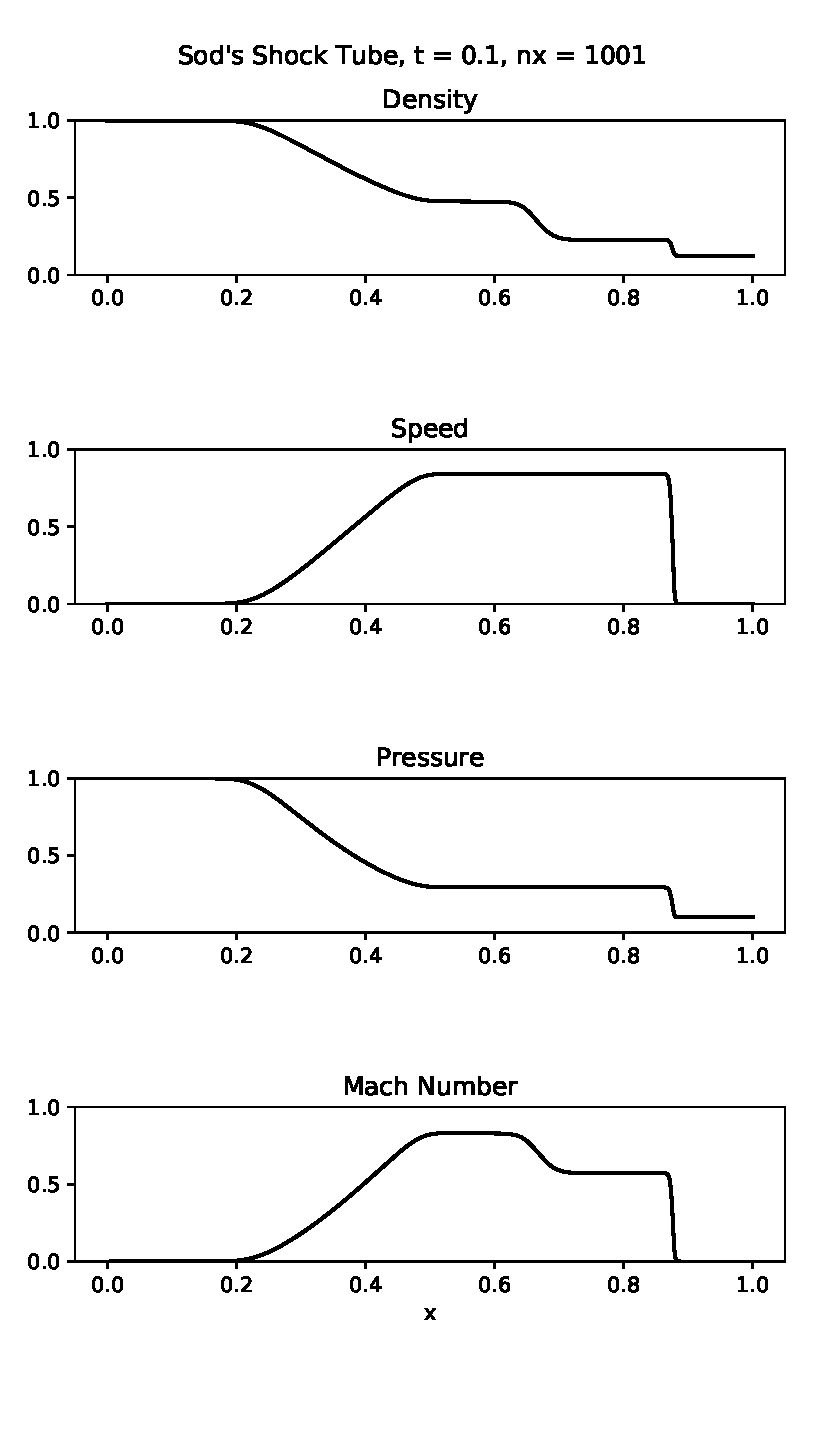
\includegraphics[width=0.75\textwidth]{images/shocktube.eps}
	\caption{Neutral fluid shock tube tests. The shocks are being captured appropriately due to the TVD-MUSCL scheme used.}\label{fig:shocktube}
\end{figure}

\citet{Soler2013} devised an initial value problem to test Alfv\'en waves in partially ionized plasmas. In the paper two-fluid plasma dynamics were explored in many ways. Analytical derivations and wave mode derivations were made. The initial value problem posed by~\citet{Soler2013} is based on their fundamental standing mode of an Alfv\'en wave in the fully ionized case of $\omega L / V_A = \pi / 20$. This means in the simulation domain of $z = (-10L,10L)$ an initial value for the velocity perturbation is:
\begin{equation}\label{eq:solerintial}
	V_{\perp}(t=0,z) = \cos{(\frac{\pi}{20 L} z)}
\end{equation}

\begin{figure}[ht!]
	\centering
	\includegraphics[width=1\textwidth]{images/soler.eps}
	\caption{The \citet{Soler2013} initial value problem tests. Velocity is taken at $z=0$ of the standing Alf\'ven wave. The solid red is the ion velocity, the dashed blue line is neutral velocity. The top row is where the initial neutral velocity is the same as the ion velocity and the bottom row is where the initial neutral velocity is at zero. The results resemble reasonably well the tests in the \citet{Soler2013} paper.}\label{fig:soler}
\end{figure}

\begin{figure}[ht!]
	\centering
	\includegraphics[width=1\textwidth]{images/soleretal2013.png}
	\caption{Taken from \citet{Soler2013}. Compare with above (Figure~\ref{fig:soler}) for validation.}\label{fig:soleretal2013}
\end{figure}

The left and right boundary conditions in this case are set at $V_{\perp} = 0$ for both ions and neutrals. Constant and arbitrary for all other values. Three different orders of magnitude of the collision rate was used for two different cases. The first with a neutral initial value the same as the ions $V_{\perp} = U_{\perp}$ and the other where $U=0$. The results in Figure~\ref{fig:soler} show the results at $z=0$ and the Alfv\'en wave can be seen clearly damped in the cases. Note how at $\nu_{ni}=1$ the medium is moving in unison but still being damped. It is also important to note the equations used to solve this are fundamentally different than the ones in~\citet{Soler2013}. They solve for the primitive variables while CoMFi solves the conservative form. Still the graphs look similar (Figure~\ref{fig:soleretal2013}) which helps with the case of the validation of the code.
\section{Visualization}\label{sec:visualization} 

CoMFi comes with its own visualization suite written in Python using Matplotlib~\citep{Hunter2007}. The data is saved in the HDF5 file format~\citep{hdf5} which is compatible with many other visualization software, however the bundled \code{plot-scripts} folder contains the file \code{comfi.py} when imported gives tools to make plots and even animations.

\subsection{Storage}

CoMFi uses the HDF5 file format to store the data. The data hierarchy is shown in Table~\ref{tab:datahierarchy}. Other software like Origin, IDL or Tecplot may be easily used with this format. The data found in each variable is a matrix of the form, $u[x, {nz}-z]$, where ${nz}$ is the number of grid cells in height. This was chosen so the matrix is displayed properly if shown in matrix form. Some software will require the matrix to be flipped when plotted.

\begin{table}[h]\label{tab:datahierarchy}
\centering
\caption[CoMFi.hdf5 data hierarchy]{The HDF5 data hierarchy of the CoMFi code, this may be used in any visualization software with HDF5 support like IDL\@. All data is normalized. The \code{time-step} parent data name is referring to the time step of interest in the data. The \code{constant} name refers to the constant of interest with proper capitalization.}
\begin{tabular}[]{l  c  r}
	\toprule
	Time Vector & \code{/t} \\
	Normalization Constants & \code{/norm/[constant]} \\
	Ion Density & \code{/[time-step]/Np} \\
	Neutral Density & \code{/[time-step]/Nn} \\
	Ion Momentum (Horizontal) & \code{/[time-step]/NVx} \\
	Ion Momentum (Vertical) & \code{/[time-step]/NVz} \\
	Ion Momentum (Perpendicular) & \code{/[time-step]/NVp} \\
	Neutral Momentum (Horizontal) & \code{/[time-step]/NUx} \\
	Neutral Momentum (Vertical) & \code{/[time-step]/NUz} \\
	Neutral Momentum (Perpendicular) & \code{/[time-step]/NUp} \\
	Ion Temperature & \code{/[time-step]/Tp} \\
	Neutral Temperature & \code{/[time-step]/Tn} \\
	Magnetic Field (Horizontal) & \code{/[time-step]/Bx} \\
	Magnetic Field (Vertical) & \code{/[time-step]/Bz} \\
	Magnetic Field (Perpendicular) & \code{/[time-step]/Bp} \\
	Electron Temperature (Optional) & \code{/[time-step]/Te} \\
	Electron Pressure (Optional) & \code{/[time-step]/Pe} \\
	Ion Energy (Optional) & \code{/[time-step]/Ep} \\
	Neutral Energy (Optional) & \code{/[time-step]/En} \\
	\bottomrule
\end{tabular}
\end{table}

\subsection{Python Plot Scripts}

In folder, \code{plot-scripts}, the python scripts required to make several plots are shown as examples. As well as examples required to make animations into \code{mp4} file format. This is done using Matplotlib and h5py for reading the HDF5 files. The Python header to import is \code{plot-scripts/comfi.py} and the functions are well documented using the PEP8 standard.

\chapter{Chromosphere Dynamics}\label{chap:chromosphere} 

The base of the solar atmosphere (right above the photosphere), referred to as the chromosphere, is highly dynamic and is strongly influenced by magnetic field activities \citep{Hasan08}. It is partially ionized, with as much as a thousand times more neutral Hydrogen than ions \citep{Alissandrakis2018}. \citet{Song2011} and \citet{Leake2014} discussed in detail the effects of ion-neutral coupling in  the chromosphere by considering neutrals and collisions into the momentum and Maxwell equations. A local-scale configuration commonly used in chromosphere models are so-called supergranules, convection cells of 30 Mm in the horizontal directions. Supergranules are separated by strong magnetic field regions, referred to as networks. It is believed that the network regions correspond to strong magnetic field at the photosphere altitude. Because the thermal pressure decreases with height while the total magnetic flux is conserved, the magnetic field tends to expand in higher altitudes to form a canopy or `wine glass' shaped magnetic geometry so that total pressure, the  magnetic pressure, $p_B$, plus thermal pressure, $p_T$, i.e., $p_T+p_B$, is balanced at each height \citep{gabriel1976}. This geometry is reflected in a significant altitudinal change in the plasma beta, which is the ratio of the thermal to magnetic pressures, $\beta=p_T/p_B$. The chromosphere has much lower temperature than that of the hot corona. The average temperature of the Chromosphere is around 6000 K while the coronal temperature is over million degrees \citep{AvrettLoeser2008}. This dramatic change in the temperature, taking place in a very narrow region of a few hundred kilometers referred to as the transition region, known as the coronal heating problem and it is a long-standing problem in solar physics.

In the chromosphere shocks often observed and jets are commonplace in the form of spicules. Spicules are local, hot upward jets of plasma observed in the corona. The origination and mechanism behind spicule formation is not well known. Spicules are categorized into two types \citep{Pontieu2007}. Type I spicules have longer lifetimes and are typically larger (5 min and $\sim$15 Mm). Type II spicules have shorter lifetimes and are smaller ($\leq$2 min and $\sim$6 Mm). \citet{Pontieu2004} suggested that photospheric oscillations give birth to spicules. It was also suggested that magnetic reconnection may be the cause of Type II spicules \citep{Pontieu2007}.

There is strong observational evidence for the ubiquity of Alfv\'en waves in the sun's atmosphere \citep{Mathioudakis2013,McIntosh2011,Jess2009,Ofman2008,Aschwanden1999,Nakariakov1999}. These observations of the solar limbs show Alfv\'en waves with amplitudes in the range of 5-25 km/s and phase speeds 250-500 km/s.  \citet{Pontieu2007} have shown that Alfv\'en waves are carried by spicules with significant amplitudes of order 20 km s$^{-1}$. It has been suggested that Alfv\'en waves could be damped in the chromosphere due to collisions between plasma ions and neutrals and causes sufficient heating \citep{Song2011} and \citep{Song2014}. \citet{Song2017} further proposed that the nonuniform heating associated with the Alfv\'en waves may explain the formation of the spicules. \citet{Khomenko2017} looks at other waves as well as Alfv\'en waves and their effects in weakly ionized solar plasma. %chktex 8

Recent simulations and models of the chromosphere have adopted a single-fluid approach~\citep{Kuzma2017,Ni2016,BradyArber2016,Gudiksen2011}. In order to account for neutrals' effect on the plasma and electric field an `ambipolar diffusion' term is added to the Generalized Ohm's Law to account for collisions~\citep{Martinez-Sykora2012,Martinez-Sykora2017}. This is useful to study the highly magnetized, low $\beta$, environment of the upper chromosphere. A two-fluid approach takes into account separate fluid motions of plasma and neutrals especially in highly collisional environments like the low solar atmosphere in regions of high magnetic gradients. \citet{Soler2013} studied Alfv\'en wave propagation in partially ionized plasma while taking a generalized approach with free parameters with the lower solar atmosphere case as an example. \citet{Maneva2017} and \citet{Wojcik2018} studied acoustic wave propogation using a collisional two-fluid approach as well. Three-fluid simulations, with electrons being the third fluid, were made to study reconnection events in the chromosphere~\citep{Leake2013}. In these highly localized small regions electron motion is seperate from ion and neutral motion and its effects cannot be neglected. The previously mentioned work uses the {\it Bifrost\/} \citep{Gudiksen2011} code which employs a very large artificial viscosity for stability. By self-consistently solving plasma, neutral fluids, and Maxwell's equations, \citet{Tu2013} have shown that due to Joule dissipation Alfv\'en waves can provide strong enough chromospheric heating and that the heating rate is consistent with the theoretical model of \citet{Song2011}.

\section{Governing Equations}\label{sec:governingeq}

In the model presented here, a two-fluid, collisional approach is used to account for the friction between ions and neutrals. The first fluid, the ion fluid, is similar to the traditional, single-fluid plasma, and assumes charge quasi-neutrality. With the Maxwell's equations, this fluid is used to calculate self-consistently the evolution of the plasma motion, magnetic fields and currents in the system. The second, neutral fluid, accounts for the neutral particles in the system. The two fluids interact by collisions. The friction between ions and neutrals affects the neutral fluid motion so that the neutrals experience the electromagnetic effects. 

This is similar to the three-fluid HiFi code used for studying reconnetion in the chromosphere \citep{Leake2012}. Except electrons are not treated as a separated fluid in this model because the electron's mass is more than three orders of magnitude smaller than ion or neutral particle mass, so its contribution to heating and the equations considering the scales is negligible. The effects of its motion are included in the current terms. We use empirical number density model that comes from observations assuming steady-states in the chromosphere~\citep{AvrettLoeser2008}. Here, I do not account for ionization and recombination which I plan to implement photo-chemistry in future work.

Our model uses Cartesian, 2.5 dimensionality, which means that all the quantities are functions of horizontal ($x$) and vertical ($z$) directions but uniform in the $y-$ direction, while vector quantities  have all three components including the third component that is perpendicular ($\perp$) to the $x-z$ plane. The perpendicular components are used to generate Alfv\'en waves at the photospheric boundary. 

The governing equations are adapted from \citet{Tu2016} for the two-fluid (plasma and neutral) system as follows:

\begin{equation}
	\frac{\partial \rho_i}{\partial t} + \nabla \cdot \rho_i \textbf{V} = 0
\end{equation}

\begin{equation}
	\frac{\partial \rho_n}{\partial t} + \nabla \cdot \rho_n \textbf{U} = 0
\end{equation}

\begin{equation}\label{eq:plasmamomentum}
	\frac{\partial \rho_i \textbf{V}}{\partial t} = - \nabla \cdot [\rho_i \textbf{VV} + n_i k_b T_i + \frac{B^2}{2 \mu_0}\textbf{I} - \frac{\textbf{BB}}{\mu_0}] + \rho_i \textbf{g} - \rho_i \nu_{in} (\textbf{V} - \textbf{U})
\end{equation}

\begin{equation}\label{eq:neutralmomentum}
	\frac{\partial \rho_n \textbf{U}}{\partial t} = - \nabla \cdot [\rho_n \textbf{UU} + n_n k_b T_n] + \rho_n \textbf{g} + \rho_i \nu_{in} (\textbf{V} - \textbf{U})
\end{equation}

\begin{equation}
	\frac{\partial \textbf{B}}{\partial t} = - \nabla \cdot ( \textbf{VB} - \textbf{BV} ) - \nabla \times ( \eta \textbf{J}  + \frac{1}{n_e e} \textbf{J} \times \textbf{B} )
\end{equation}

\begin{equation}\label{eq:energyion}
\begin{aligned}
	\frac{\partial k_b T_i}{\partial t} = - \nabla \cdot (k_b T_i \textbf{V}) + \frac{1}{3} k_b T_i \nabla \cdot \textbf{V} - \frac{2}{3} \frac{\nabla \cdot (\textbf{q}_i + \eta \textbf{B} \times \textbf{J})}{n_i} \\
	+ \frac{2}{3} \frac{m_i}{m_i+m_n} \nu_{in} [3 k_b (T_n - T_i) + m_n | \textbf{V} - \textbf{U} |^{2} ]
\end{aligned}
\end{equation}
\begin{equation}\label{eq:energyneutral}
\begin{aligned}
	\frac{\partial k_b T_n}{\partial t} = - \nabla \cdot (k_b T_n \textbf{U}) + \frac{1}{3} k_b T_n \nabla \cdot \textbf{U} - \frac{2}{3} \frac{\nabla \cdot \textbf{q}_n}{n_n} \\
	+ \frac{2}{3} \frac{m_n}{m_i+m_n}  \nu_{in} [ 3 k_b (T_i - T_n) + m_i | \textbf{V} - \textbf{U}|^{2} ]
\end{aligned}
\end{equation}

\begin{equation}
	\nabla \times \textbf{B} = \mu_0 \textbf{J}
\end{equation}

\begin{equation}
	\textbf{q} = - \kappa \nabla T
\end{equation}

Here $i$, $e$ and $n$ subscripts denote proton, electron and neutral, respectively. The primitive scalars $m$, $\rho$, $T$ are particle mass, mass density and temperature, respectively. $\textbf{V}$, $\textbf{U}$, and $\textbf{B}$ are ion velocity, neutral velocity, and the magnetic field, respectively, with $\textbf{g}$ denoting the solar gravitational acceleration near the solar surface. $\kappa$ is the Spitzer conductivity. $\nu_{ij}$ denotes collision rate of species $i$ to species $j$, and $\eta = m_e(\nu_{en} + \nu_{ei})/e^2n_e$ is the ohmic resistivity. We use the following collision rates \citep[see][Appendix A]{Pontieu2001} 
\begin{eqnarray}
&\nu_{in} = 7.4 \times 10^{-11} n_n T^{1/2}& \nonumber\\
&\nu_{en} = 1.95 \times 10^{-10} n_n T^{1/2}& \\
&\nu_{ei} = 3.759 \times 10^{-6} n_e T_e^{-3/2} \ln \Lambda& \nonumber
\end{eqnarray}
where $\ln \Lambda$ is the Coulomb logarithm taken as 10 for simplicity and $n$ is in cm$^{-3}$ and $T = \frac{T_i + T_n}{2}$ in K.

Comparing this with the two-fluid equations seen in Section~\ref{sec:2fluidmhd} we see that we've taken the more extreme case of $m_e \sim 0$. This is for the first-order approximation that electrons contribute less to heating than hydrogen ions and neutrals. The CoMFi code is capable of reverting back to the approximation, $\frac{m_e}{m_i} \sim 0$, for cases where the current density terms matter like in mid-chromosphere reconnection.

\section{Simulation Domain}\label{sec:simulationdomain}

In the horizontal dimension, I simulate a supergranule similar to that described in \citet{Song2017}. Because of symmetry, our simulation domain contains half of a supergranule, from the center of a network with strong field to the center of internetwork at the photospheric boundary. If I further assume that the neighboring supergranules have the same polarity as the one in the simulation domain, there is no reconnection between the supergranules of interest.  In this case  the normal component of the field, $B_x$, is zero at the left and right boundaries. The right and left boundaries act as mirrors to reflect any normal component of the field. Similarly, the normal component of the velocity is also set to zero at the right and left boundaries, i.e.\ there is no horizontal flow from one supergranule to another at the chromospheric altitude although inter-supergranule flow is possible in the corona height and in or below the photosphere. 

Since I only simulate the chromosphere and treat the transition region above and photosphere below as upper and lower boundaries, respectively. The photosphere below is made up as a Dirichlet boundary conditions below the surface of the photosphere, the sun is highly dynamic. The assumption made in this mode is the Alfv\'en waves are generated at the photosphere and propagate while undergoing damping towards the transition region. For this reason to imitate the energy flux and activity of the photosphere, a driver at the bottom of the simulation domain is made as a Dirichlet boundary condition. Using the broadband spectrum driving method of \citet{Tu2013}, the perpendicular velocity is a continuous oscillation with a broadband time series of the form:

\begin{equation}
\begin{aligned}
	V_{\perp} (t, z=0) = V_b [ \sum_{k=0}^s {(\omega_k/\omega_p)}^{5/6} \cos{(\omega_k t + \Phi_k)} \\
	+ \sum_{j=s+1}^m {(\omega_p/\omega_j)}^{5/6} \cos{(\omega_j t + \Phi_j)} ]
\end{aligned}
\end{equation}

where $V_{\perp}$ will be the imposed speed on the lower boundary in the direction normal to the $x-z$ plane. $V_b$ is the amplitude of the broadband spectrum, 2 km/s, to ensure an appropriate photospheric flux of $2 \times 10^7$ erg cm$^{-2}$ s$^{-1}$ \citep[see][section 3.2]{Tu2013}, $\omega_j$ and $\omega_k$ are angular frequencies filled logarithmically, $\omega_p$ is the peak angular frequency at 1.65 mHz. The driver also has random phases $\Phi_j, \Phi_k$ which is a multiple of 2$\pi \times$ by random number between 0 and s+m. For the case of this simulation s=100 and m=500. 

The number density of the ions and neutrals are specified at the boundary as the photospheric values from \citet{AvrettLoeser2008} of 10$^{20}$ m$^{-3}$ and 10$^{23}$ m$^{-3}$, respectively. As an initial condition, a stratified hydrostatic profile is made for the ion densities $n(z) = n(z=0) e^{-m_{i}gz/kT_0}$ and a more realistic neutral number density profile is filled based on the above mentioned model. Here T$_0$ = 7000 K which is the temperature imposed on the photosphere and also the initial condition for both ionized plasma and neutrals in the entire domain. An isothermal approach was chosen initially because the chromosphere's temperature does not change much, between 6000K to 8000 K, between the photosphere and the transition region. At later times, the temperatures are determined from the energy equations~\ref{eq:energyion} and~\ref{eq:energyneutral}. 

A requirement in some MHD codes with zero magnetic field divergence constraints is that the initial condition must also be divergence free. For this reason $B_x(t=0)$ and $B_\perp(t=0)$ is chosen to be zero while $B_z(x, t=0)$ varies in the horizontal $x$ direction. It consists of regions of strong field, $\sim$1kG, for the network region and weak fieild, $\sim$50 G, for the internetwork region with a sharp linear drop in between. The 1 kG region only takes up 0.05 Mm in the horizontal direction and is in the left part of the domain. The weak region part of the rest of the domain. The goal is to allow this initial condition to quickly relax to a canopy because of the large $\beta$ change due to height without solving a force-free field. At the bottom boundary,  a Dirichlet condition is applied to $B_z(x)$ but for the other two components the field is set Neumann conditions $\frac{\partial B_{z,\perp}}{\partial z}\vline_{z=0km} = 0$. This configuration resembles the stem of the canopy and the magnitude of the supergranule strengths at the photosphere. The bottom boundary's $B_z(x)$ is an unchanging Dirichlet condition to mimic the convection cell underneath.

At the top boundary which represents the transition region and the corona above it, the model uses Neumann conditions to allow free-flow of the plasma through it (i.e. $\frac{\partial \textbf{u}}{\partial z}\vline_{z=2100km} = 0$).

In the simulations and results shown in this paper the domain is 15 Mm horizontally (half the size of the magnetic internetwork) and 2.1 Mm vertically (typical thickness of the chromosphere). It is a uniform Cartesian grid of 256$\times$128 where $\Delta x = 58.6$ km and $\Delta z = 16.4$ km. This is the largest resolution chosen for speed and memory considering the usage of a dedicated scientific computing GPU (see Chapter~\ref{chap:implementation}). This is larger than the length scale of the collisionally reduced Alfv\'en wavelength ($\frac{V_A}{\nu_{in}}$) which means for this simulation the plasma and neutrals are coupled. Since this is a 2.5D simulation all spatial derivatives in the perpendicular direction are taken as zero ($\frac{\partial}{\partial \perp} = 0$).

All momentum components are set initially as zero.

\section{Results}\label{sec:results}

Figure~\ref{fig:granulegeometry} shows a snapshot on the chromospheric solution after $348~ms$. It shows that our simulation produces magnetic field topology that is characterized by canopy or `wine glass' shape \citep{Rutten2007}, with a strong field of about $1~kG$ at the stem on the left, and a weaker field of about $50~G$ at the near the upper boundary of the simulation domain, near the transition region.  This topology is obtained fairly quickly, in around $\sim$350ms, because of the magnetic pressure imbalance imposed in the initial conditions. This is not a relaxed system as the canopy holds for a few seconds before an eruption starts forming. 

\begin{figure}[ht!]
	\centering
	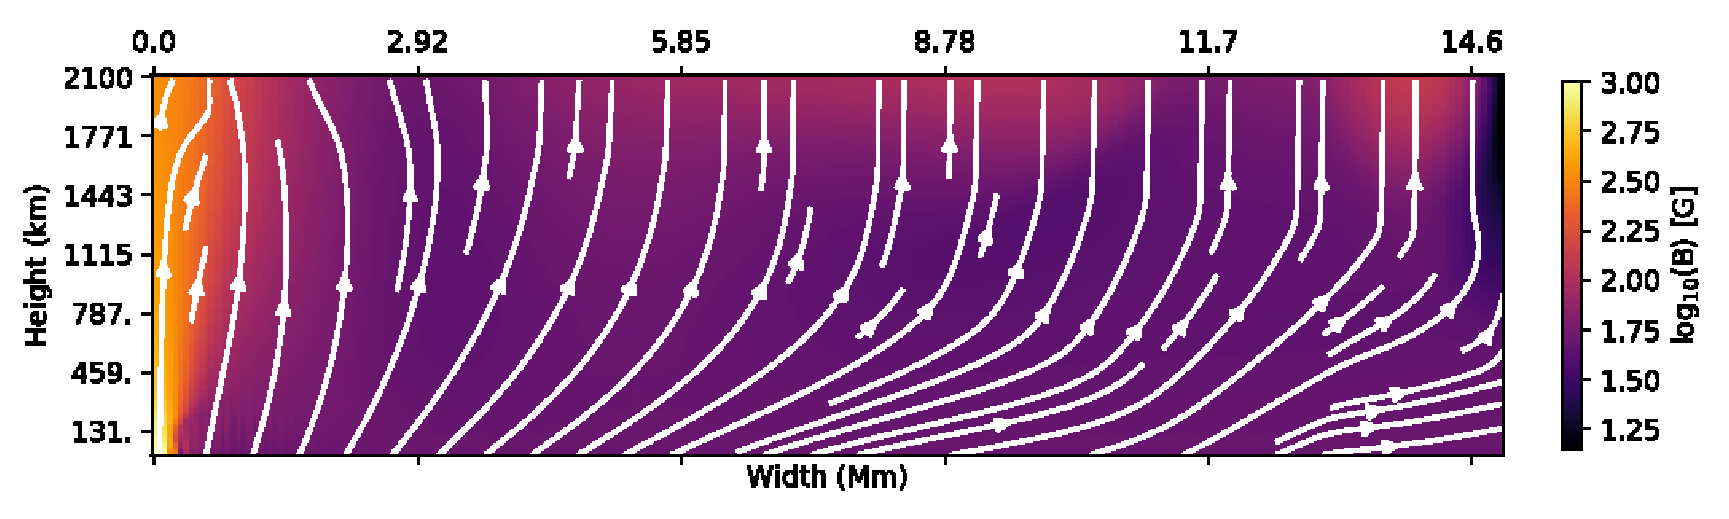
\includegraphics[width=1\textwidth]{images/granulegeometry.eps}
	\caption{Formation of a canopy seen after around 348ms (13000 time steps). The initial condition of a concentrated strong field region (1 kG) and weak field region (5G) creates vertical asymmetry as plasma beta drastically decreases. The left and right boundaries are mirrored so effects of other granules behaving the same way are considered. Because of the short time period this is \textit{not} a relaxed system but simply a consequence of the pressure imbalance frequently seen in the chromosphere.}\label{fig:granulegeometry}
\end{figure}

Figure~\ref{fig:spiculeshock} shows a formation of what resembles a jet --- a parcel of plasma quickly moving upward towards the transition region. The shock spontaneously forms after around 20s and the jet speeds up and shoots up outside of the chromosphere into the corona in about 5s. 

\begin{figure}[ht!]
		\centering
		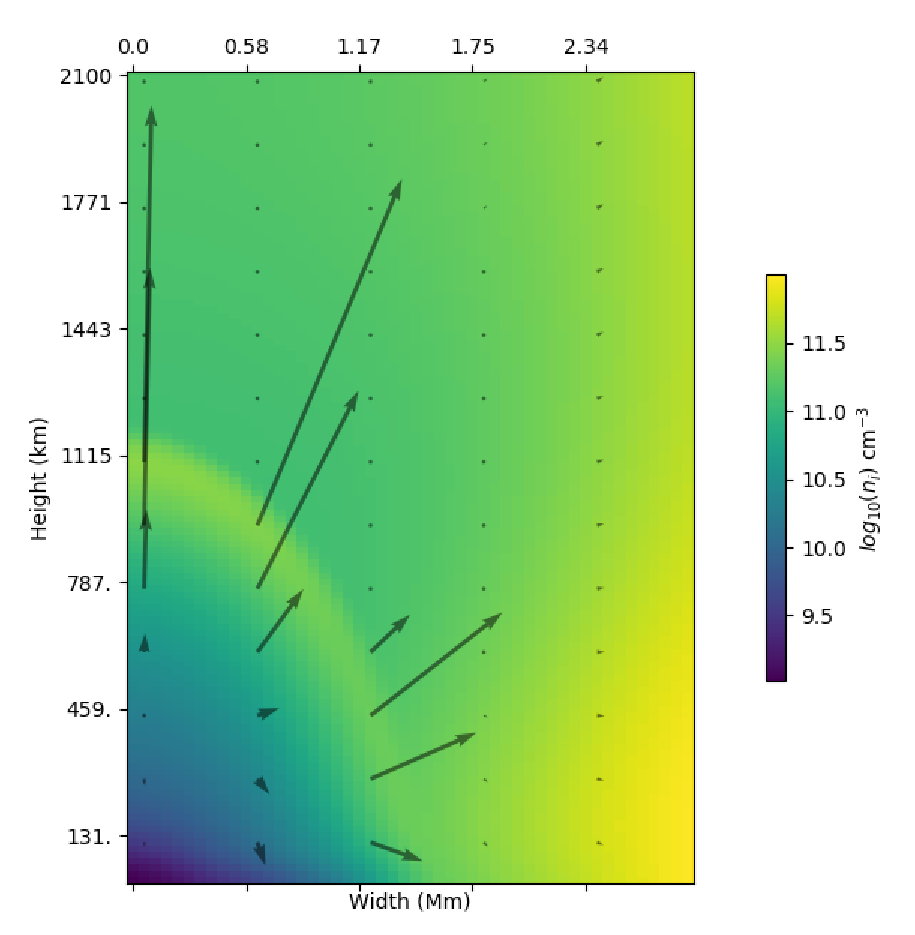
\includegraphics[width=0.6\textwidth]{images/spiculeshock.eps}
		\caption{A zoom into the shock wave front of the jet. The arrows represents the direction and magnitude of ion flow. The color bar represents the neutral number density in cm$^{-3}$}\label{fig:spiculeshock}
\end{figure}

In Figure~\ref{fig:prespicule}, I show the distribution of the two heating terms---the ohmic heating, $\eta J^2$, and the frictional heating, $\nu_{in} \rho_i |\textbf{V} - \textbf{U}|^2$, in the simulation domain, right before the eruption. The heating rates are normalized per neutral particle. It can be seen that the frictional heating dominates the ohmic heating by orders of magnitude, especially in the strong field region where the shock forms.

\begin{figure}[ht!]
    \centering
    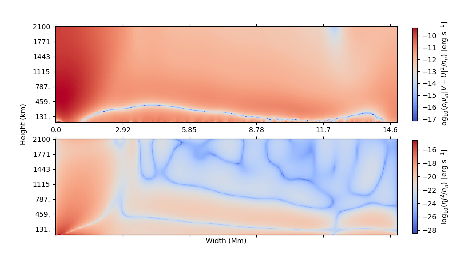
\includegraphics[width=1\textwidth]{images/prespicule.eps}
    \caption{Heating of the shock origin before the formation of the jet at t=18.9s. Top image is the frictional heating per neutral particle. Bottom image is the ohmic heating per neutral particle. The frictional heating is orders of magnitude larger than the heating due to currents.}\label{fig:prespicule}
\end{figure}

Figure~\ref{fig:midspicule} shows the neutral temperature, the frictional heating, and the velocity difference, $| \textbf{V} - \textbf{U}|^2$ during the emergence of the jet to the corona (at $t=26.8~s$). The plots show the formation of an appreciable shock which separates a low number density, high temperature and strong heating region with a high number density, lower temperature and weaker heating with the rest of the medium. The figure also shows a very clear difference in heating rates on both sides of the shock, where the front of the shock travels at super sonic speeds. The shock propagates supersonically until the plasma is ejected when the chromosphere is depleted and starts to fill up again with flows going back down. Downstream of the shock, the plasma flow is returning due to a cavity left behind, where upstream of the shock, the chromospheric plasma is still unchanged.

\begin{figure}[ht!]
	\centering
    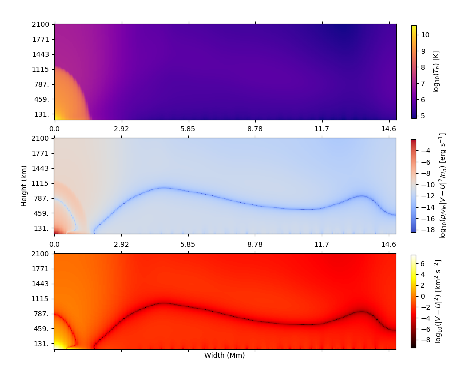
\includegraphics[width=1\textwidth]{images/midspicule.eps}
	\caption{These figures show the jet in the middle of its journey to the corona at t=26.8s. From top to bottom, the temperature of the neutral plasma, the frictional heating per neutral particle, and the difference in speeds $\| \textbf{V} - \textbf{U} \|^2$ of the charged and neutral plasma. The shock can be clearly seen in the bottom-left corner of the simulation where the magnetic flux concentration is strongest. Due to large plasma beta a `ring' of slow moving plasma is formed and persists in the shock allowing the shock to start forming.}\label{fig:midspicule}
\end{figure}

Figure~\ref{fig:spiculetimeseries} shows a time series of the evolution of the shock number density and magnetic field lines. It can be seen that the field lines follow the shock evolution, which means magnetic field topology (i.e., reconnection region) is not a driver of the jet. Figure~\ref{fig:heatingtimeseries} shows the same time series but with contours of frictional heating and flow streamlines. It clearly shows that the jet is driven by frictional joule heating.

\begin{figure}[ht!]
	\centering
    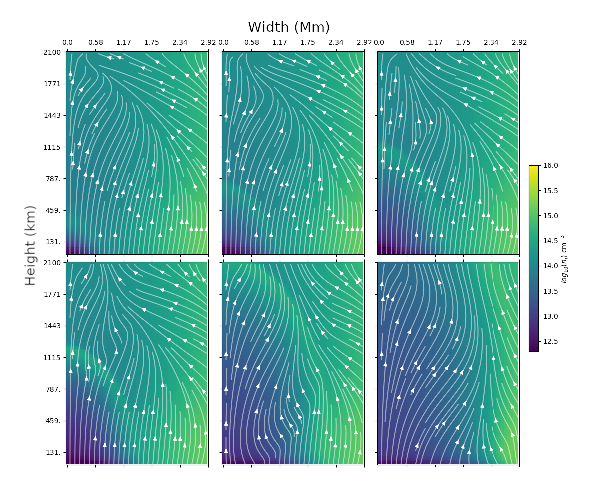
\includegraphics[width=1\textwidth]{images/spiculetimeseries.eps}
    \caption{Time series of the shock. From left to right and top to bottom the times are t=26.751s, 26.785s, 26.831s, 26.842s, 26.844s, 26.849s. The white streamlines denote the magnetic field lines and the number density of the neutrals are in cm$^{-3}$. This shows them magnetic field geometry changing due to the jet and not the other way round. The jet is not generated because of the magnetic field.}\label{fig:spiculetimeseries}
\end{figure}

\begin{figure}[ht!]
	\centering
    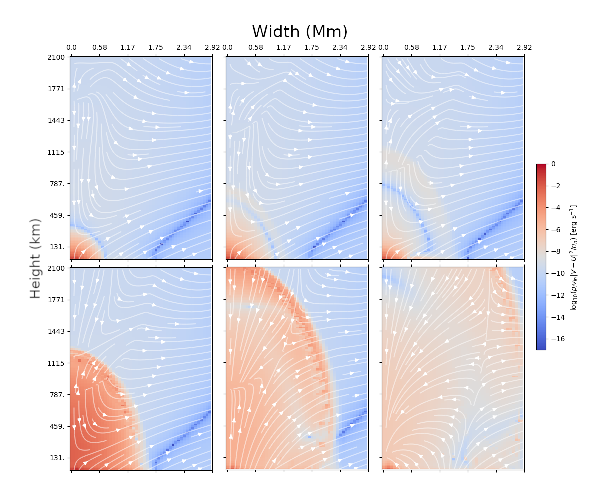
\includegraphics[width=1\textwidth]{images/heatingtimeseries.eps}
    \caption{Time series of frictional heating in the jet. From left to right and top to bottom the times are t=26.751s, 26.785s, 26.831s, 26.842s, 26.844s, 26.849s. The white streamlines denote flow.}\label{fig:heatingtimeseries}
\end{figure}

Figures~\ref{fig:shockwavefront1d},~\ref{fig:spiculefield1d},~\ref{fig:spiculefriction1d} and~\ref{fig:spiculespeed1d} show one-dimensional extractions of the solution during the shock emergence along a vertical line at $x=0.6~Mm$.  These plots exemplify the cause and effect of the shock. The first plot shows the time series of the wavefront of the shock climbing in the chromosphere. The second and third show that the frictional heating jump follows the shock, and that the magnetic field changes correspond to the jet behind the shock. The last plot shows a velocity profile of the jet.

\begin{figure}[ht!]
	\centering
    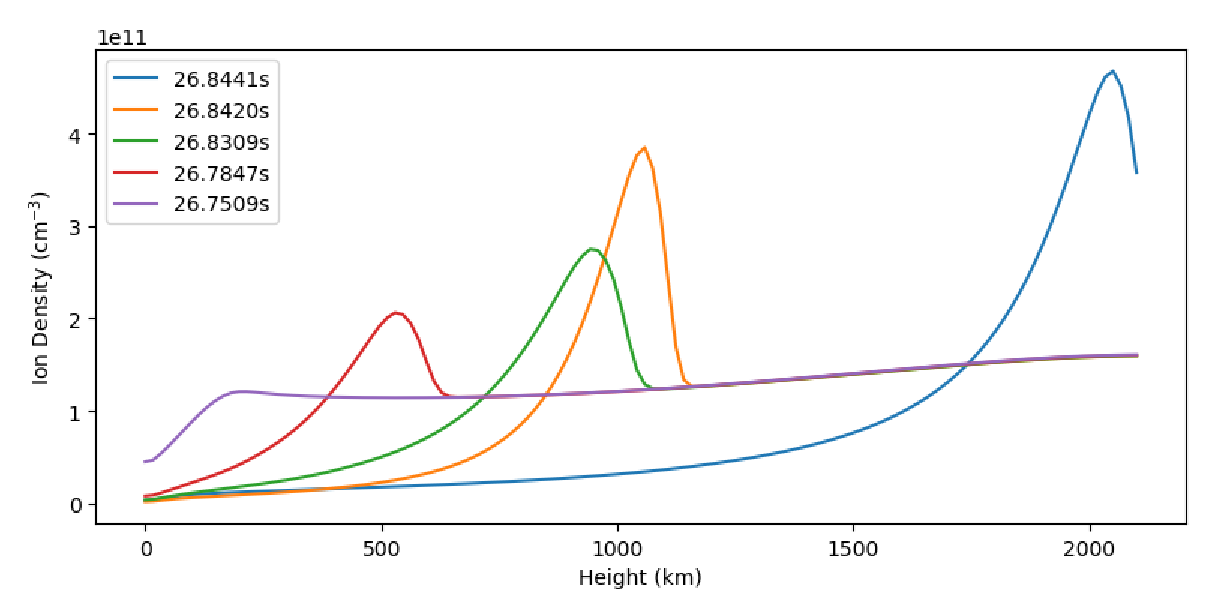
\includegraphics[width=1\textwidth]{images/shockwavefront1d.eps}
    \caption{Ion number density snapshots of shock wave front at line of extraction x=0.6Mm. Ion number density is in units of $10^{11}$ cm$^{-3}$. The wavefront can be clearly seen climbing the Chromosphere.}\label{fig:shockwavefront1d}
\end{figure}

\begin{figure}[ht!]
	\centering
    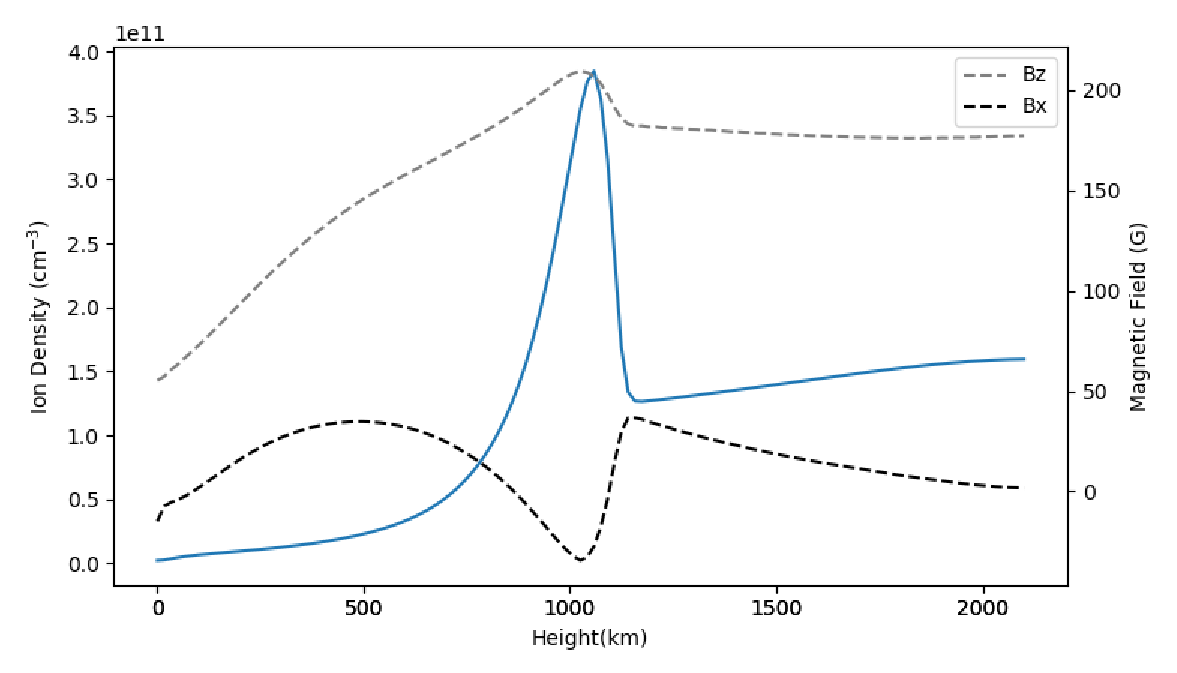
\includegraphics[width=1\textwidth]{images/spiculefield1d.eps}
    \caption{Blue line is ion number density and the black and gray dashed lines are $B_x$ and $B_z$ respectively at t=26.83s and vertical line at x=0.6Mm. Ion number density is in units of $10^{11}$ cm$^{-3}$. The magnetic field is changed behind the shock wave front.}\label{fig:spiculefield1d}
\end{figure}

\begin{figure}[ht!]
	\centering
    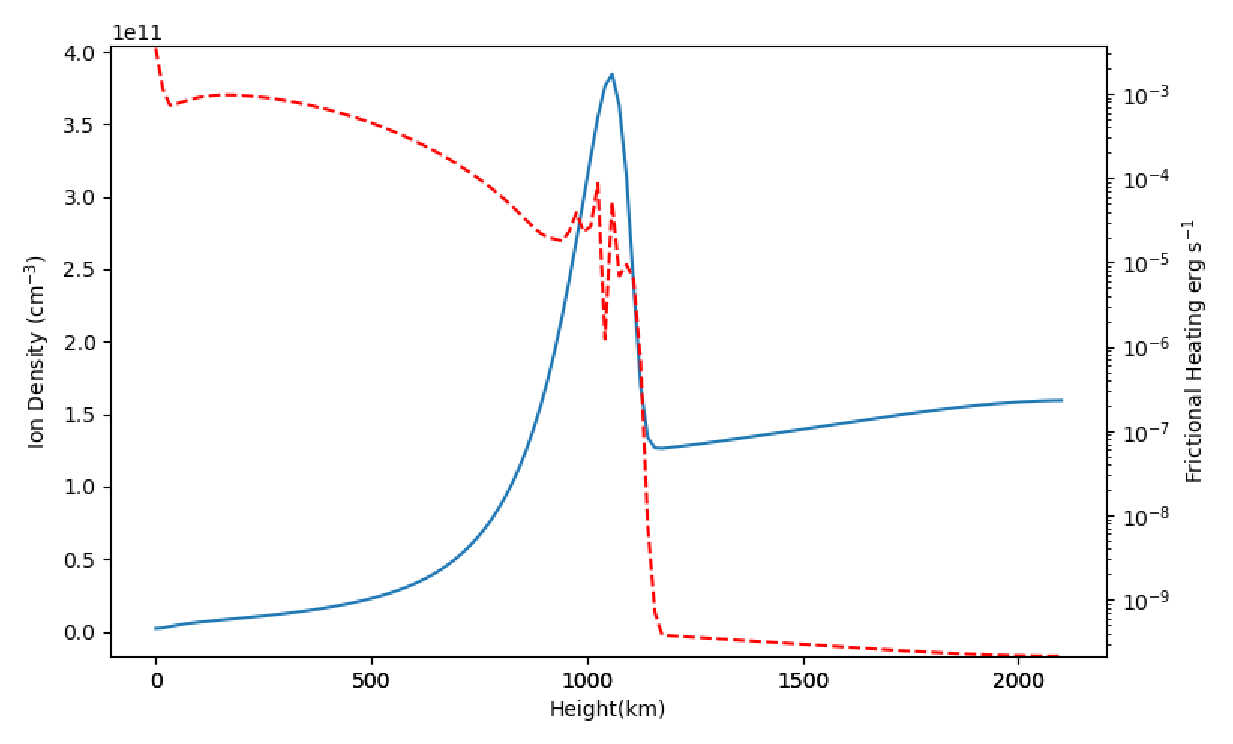
\includegraphics[width=1\textwidth]{images/spiculefriction1d.eps}
    \caption{Blue line is ion number density and red dashed line is frictional heating per neutral particle at t=26.83s and vertical line x=0.6Mm. Ion number density is in units of $10^{11}$ cm$^{-3}$. The frictional heating per neutral particle behind the wavefront is orders of magnitude higher than in front of it.}\label{fig:spiculefriction1d}
\end{figure}

\begin{figure}[ht!]
	\centering
    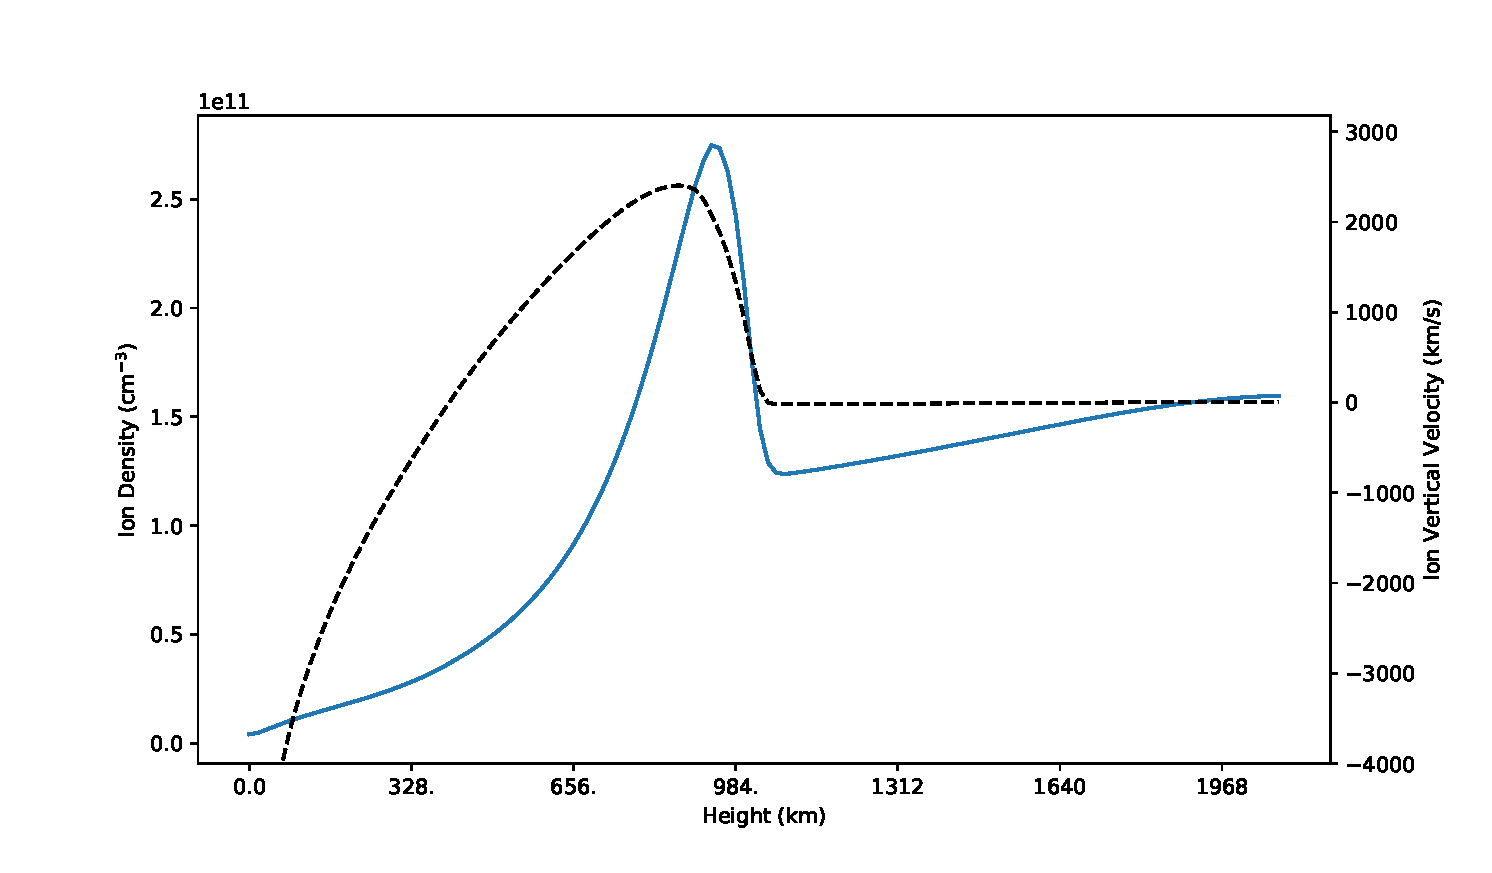
\includegraphics[width=1\textwidth]{images/spiculespeed1d.eps}
    \caption{Blue line is ion number density and black dashed line is vertical ion velocity at t=26.83s and vertical line x=0.6Mm. Ion number density is in units of $10^{11}$ cm$^{-3}$. The jet speed is supersonic.}\label{fig:spiculespeed1d}
\end{figure}

\section{Discussion}\label{sec:discussion}

A magnetic canopy forms due to the magnetic and thermal pressure imbalance of the strong field regions from the photosphere and the weak field but high temperature regions scaling up to the transition region. This is consistent with a two-fluid analytic model that was presented in \citet{Song2017}. It shows that the model can provide numerical solutions for chromospheric conditions. However, the magnetic canopy does not relax or reach a steady-state due to the nature of the collisional model and not in the timescales of the current simulation. The super granule canopy may not last because the photospheric power flux, generated at the lower boundary, continuously adds energy into the system. Small scale processes or highly dynamic events like jets override the canopy magnetic field because of large plasma speeds. Our results show that the jet has immediate effects on the magnetic field due to induction and not vice versa.

Largest Alfv\'en speeds seen in the simulation is 11 Mm/s which means that in the 30s of simulation, magnetic effects can travel through the domain at least 3 times with constant density and even less in a hydrostatic density. Alfv\'en waves generated as the drivers for frictional heating at the bottom boundary do not reflect at the top boundary enough times to warrant a time-averaged study of the entire heating of the chromosphere nor does it have enough energy to drive the jet of the same kind as presented. The presence of the shock also inhibits any long-term ideal studies of the atmosphere since it depletes and cavities form with the jet. In a future study, I will see how Alf\'ven waves affect the chromosphere with force-free initial conditions so as to not form any jets that can destroy a canopy configuration.

Although the frictional heating is large in the entire magnetic network column, an instance of no frictional heating creates a separation of upstream and downstream fluids preceding the shock. This can be seen in Figure~\ref{fig:prespicule} and~\ref{fig:midspicule} and is due to a high temperatures and density which causes the two fluids to move in unison and therefore $\rho_{in} \nu_{in} \|V-U\| = 0$. The cause of the frictional heating is not Alfv\'en wave damping but the imbalanced initial conditions and the horizontal \textbf{J} $\times$ \textbf{B} force. The lower medium heats faster than above it and this creates the shock in the lower atmosphere that then propagates due to thermal pressure.

It has been suggested that the driver of these kinds of spicule-like events is magnetic reconnection which originates from the vicinity of a large magnetic flux concentration in the network \citep{Pontieu2007}. In our simulation, the frictional heating heats a fluid downstream of the unison speed ring larger than that of upstream causing a shock wave as expected from a Type I spicule. However the simulation does not show reconnection effects with enough energy to drive a spicule. Although MHD simulations do not mimic reconnection directly, currents present in reconnection events would accelerate electrons into a collision due to the dense and hot medium surrounding it. Therefore, magnetic reconnection is directly related to ohmic heating in the chromosphere. If comparing the dominating heating terms, frictional heating dominates ohmic heating which means {\it collisions are causing these jets to form and not reconnection-like currents}. The size and extreme temperatures of the jet in the simulation closely resemble chromospheric jets~\citep{Shimojo2000,Nishizuka2011}.

In Figure~\ref{fig:shockwavefront1d} the jet can be seen accumulating a shock of number density $10^{11}$ cm$^{-3}$. This density is consistent with IRIS observations of spicules in the corona~\citep{Alissandrakis2018}. The simulation does show that changes in the magnetic field happen behind the shock wave front's direction of motion. Figure~\ref{fig:spiculefield1d} implies the change in the magnetic field is a consequence of the jet and the rising magnetic field density in the plane of the simulation is due to compression from the shock itself. The shock in the frictional heating term, $\frac{\rho_i \nu_{in} \| \textbf{V} - \textbf{U} \|^2}{n_n}$, seen in Figure~\ref{fig:spiculefriction1d} coincides exactly at the shock showing enhanced heating behind the shock front. The cause of the shock climb is the thermal pressure behind and in front of the shock.

The jet's temperatures and speed are much larger than observed. This is mostly due to the fact that in my model I have not included the radiative loss effect in the energy equations. The larger than reality shock heating because of the greater flow speed may also further amplify the temperature. The over-estimated temperature of the downstream medium may also lead to estimate of the collision frequencies. This growing downstream temperature has a compounding effect on the thermal pressure gradient downstream and upstream and causes the speeds to go supersonic. Further studies will incorporate the photo-chemistry and also radiative losses. These implementations will help to see how they affect shock formation and the energy balance inside the chromosphere. It is also important to note that this shock travels at super-Alfv\'enic speeds so it is a super-Alfv\'enic jet.

\citet{KuzmaApJ2017} made a numerical simulation of a solar spicule by imposing a vertical pulse in the solar limb. In contrast, the shock shown in our simulation self-consistently evolves without forcing a push on the plasma and the jet is a consequence of thermal effects. Thus, it provides a complete picture of the chromospheric heating conditions for shock formation. The spicule speeds in \citet{KuzmaApJ2017} match more closely to the observed $25~km~s^{-1}$ than our simulation, but that is expected in the case where the pulse is controlled and the simulation is single-fluid. \citet{KuzmaApJ2017} also investigated adiabatic and non-adiabatic studies of spicules and the wave structures found in the plasma. The jets in our simulation are different than the imposed pulses of~\citet{Kuzma2017} since that is a cold dense plasma that has been imposed, while in our simulation, it is a hot large plasma jet that evolved self-consistently.

\citet{Song2014} found that by subtracting the two fluids' momentum equations the evolution of the speed differences, $d/dt|\textbf{V}-\textbf{U}|$, which leads to frictional heating is caused and maintained by magnetic pressure and thermal pressure differences between the fluids. \citet{Tu2013}, who studied a time-averaged heating in the chromosphere, found that ohmic heating dominated the lower chromosphere and frictional heating dominated the upper chromosphere which adequately explained the heating of the chromosphere. This picture seems to be different from the results of our simulation as frictional heating dominated ohmic heating in the lower chromosphere but this is most likely due to the field strength used in the two studies. Their study limited the field in less than 100 G, but our model includes region of 1 kG field. The one order of magnitude higher in the field decreases the ohmic-to-frictional heating ratio by two orders of magnitude.

We use our model to demonstrate the importance of collisions in the chromosphere. A model without collisions is incomplete as neutral particles dominates the charged particles in this small layer of the sun. By simply adding collision terms I show that the simulation replicates chromospheric conditions well. Such a model can be used as an interface between the (fully) neutral photosphere and the (fully) ionized corona. \citet{Hillier2016} investigated 1D slow-mode shocks in chromospheric conditions and how magnetic energy can be converted to frictional heating in these cases.

Finally, this work serves as a step towards a better understanding of the solar chromosphere. The {\it Parker Solar Probe\/} mission \citep{SolarProbe16} is expected to shed light on the dominant processes in the solar atmosphere, including the chromosphere, and these processes will be implemented in the model. 

\chapter{Conclusion}\label{chap:conclusion}

MHD collissional modeling, chromospheric modeling, scientific computing, and introducing the CoMFi code were the focus of this dissertation. Typically in the world of physics, the uptake of new ideas in science is not without inertia. This is understandable as I spend our time focusing on the physics above all else. If I take Moore's Law as a metaphor, I should understand that eventually computers will be able to do whatever I please it to and relying on legacy codes will be a thing of the past. An example of this is the Python programming language. A couple decades ago I could not prototype the kind of software I am able to nowadays by the invention of this programming language. Analogously, decades from now I should be able to solve differential equations by taking new computer science inventions and hopefully with less resistance.

We present a self-consistent, two-fluid MHD model to study the chromosphere. The model includes ion-neutral interaction, which allows us to investigate the role of frictional heating in the dynamics of the chromosphere.  The very high collision rates in the partially ionized chromosphere stabilizes the code so that no numerical viscosity is needed.  

The model obtains preliminary results which require further investigation. Our simulation presents that, between network and internetwork regions, a jet could potentially be driven purely by thermal processes, especially the frictional heating, and not by magnetic reconnection. Thus, it is crucial to include the neutrals in any attempt to model the lower chromosphere.

The discrepancy between observational speeds and speeds in the simulation could be explained by the need to include the effects of photo chemical reactions in the chromosphere and the radiative losses. Further refinement of the model with photo-chemical effects, radiation and new observations from the upcoming {\it Parker Solar Probe\/} mission will lead to an improved model of the chromosphere.  

It is my hope that the CoMFi code can continue to provide good physics in the future and hopefully adapted to suit the needs of the user. GPU clusters are an attractive new frontier in scientific computing and its thousands of cores per unit is exactly suited to solve our differential equations. As GPUs become cheaper our codes must be sure to utilize them.

%%%%%%%%%%%%%%%%%%%%%%%%%%%%%%%%%%%%%%%%
\nocite{*}
\bibliographystyle{plainnat}
\bibliography{phd-dissertation}

%%%%%%%%%%%%%%%%%%%%%%%%%%%%%%%%%%%%%%%%
\appendix
\chapter{Flux Limiters}\label{app:fluxlimiters}

The CoMFi code provides several flux limiters. The pre-made flux limiters tend to be symmetric:

\begin{equation}
	\frac{\phi(r)}{r} = \phi(\frac{1}{r})
\end{equation}

This is to ensure that it is consistent in negative and positive fluxes.

The provided flux limiters are:

\begin{equation}
	\phi_{ospre} (r) = 1.5 \frac{(r^2 + r)}{r^2 + r + 1}
\end{equation}

This is the Ospre~\citep{Waterson2007} limiter, the default limiter in the code.

\begin{equation}
	\phi_{van Albada} (r) = \frac{r^2 + r}{r^2 + 1}
\end{equation}

By~\citet{vanalbada1982}.

\begin{equation}
	\phi_{van Leer} (r) = \frac{r + \lvert r \rvert}{1 + \lvert r \rvert}
\end{equation}

By~\citet{vanleer1974}

These were chosen because of ViennaCL's limitation of not having element-wise min and max functions. ViennaCL does have the ability to compile custom kernels and examples of min-mod in that case does exist.

\begin{figure}[h!]\label{fig:sweby}
	\centering
	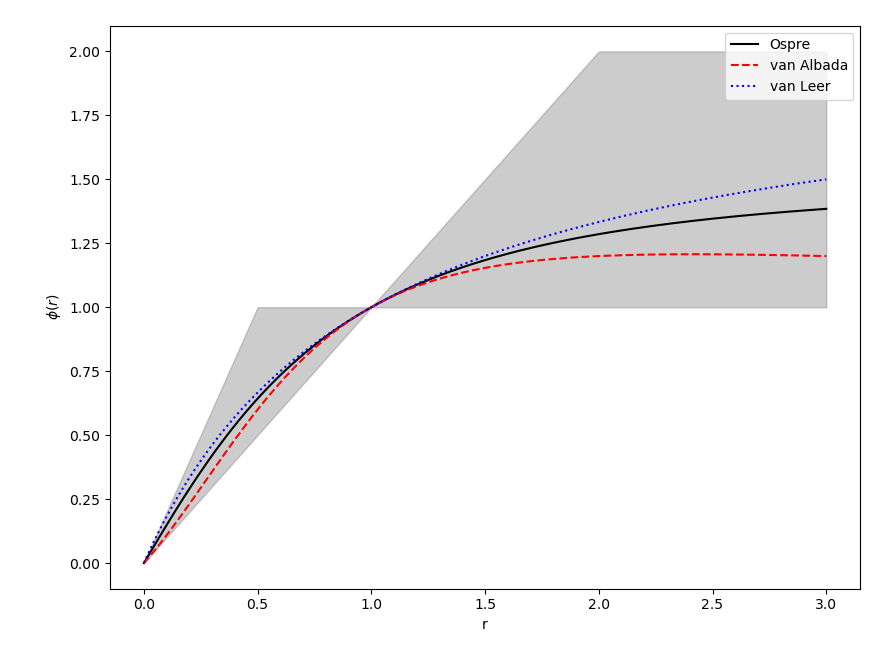
\includegraphics[width=1.0\linewidth]{images/sweby.png}
	\caption{A Sweby diagram of the current limiters in the CoMFi code. The shaded region is the required region for the limiter to be in in order to be second-order TVD\@.}
\end{figure}

Only second-order TVD limiters were chosen because when the scheme is at its high-resolution it is a second-order scheme.

\end{document}
